\PassOptionsToPackage{unicode=true}{hyperref} % options for packages loaded elsewhere
\PassOptionsToPackage{hyphens}{url}
%
\documentclass[12pt, openany]{book}
\usepackage{lmodern}
\usepackage{amssymb,amsmath}
\usepackage{ifxetex,ifluatex}
\usepackage{fixltx2e} % provides \textsubscript
\ifnum 0\ifxetex 1\fi\ifluatex 1\fi=0 % if pdftex
  \usepackage[T1]{fontenc}
  \usepackage[utf8]{inputenc}
  \usepackage{textcomp} % provides euro and other symbols
\else % if luatex or xelatex
  \usepackage{unicode-math}
  \defaultfontfeatures{Ligatures=TeX,Scale=MatchLowercase}
\fi
% use upquote if available, for straight quotes in verbatim environments
\IfFileExists{upquote.sty}{\usepackage{upquote}}{}
% use microtype if available
\IfFileExists{microtype.sty}{%
\usepackage[]{microtype}
\UseMicrotypeSet[protrusion]{basicmath} % disable protrusion for tt fonts
}{}
\IfFileExists{parskip.sty}{%
\usepackage{parskip}
}{% else
\setlength{\parindent}{0pt}
\setlength{\parskip}{6pt plus 2pt minus 1pt}
}
\usepackage{hyperref}
\hypersetup{
            pdftitle={Philosophical Ethics},
            pdfauthor={George W. Matthews},
            pdfborder={0 0 0},
            breaklinks=true}
\urlstyle{same}  % don't use monospace font for urls
\usepackage[margin=3cm]{geometry}
\usepackage{longtable,booktabs}
% Fix footnotes in tables (requires footnote package)
\IfFileExists{footnote.sty}{\usepackage{footnote}\makesavenoteenv{longtable}}{}
\usepackage{graphicx,grffile}
\makeatletter
\def\maxwidth{\ifdim\Gin@nat@width>\linewidth\linewidth\else\Gin@nat@width\fi}
\def\maxheight{\ifdim\Gin@nat@height>\textheight\textheight\else\Gin@nat@height\fi}
\makeatother
% Scale images if necessary, so that they will not overflow the page
% margins by default, and it is still possible to overwrite the defaults
% using explicit options in \includegraphics[width, height, ...]{}
\setkeys{Gin}{width=\maxwidth,height=\maxheight,keepaspectratio}
\setlength{\emergencystretch}{3em}  % prevent overfull lines
\providecommand{\tightlist}{%
  \setlength{\itemsep}{0pt}\setlength{\parskip}{0pt}}
\setcounter{secnumdepth}{5}
% Redefines (sub)paragraphs to behave more like sections
\ifx\paragraph\undefined\else
\let\oldparagraph\paragraph
\renewcommand{\paragraph}[1]{\oldparagraph{#1}\mbox{}}
\fi
\ifx\subparagraph\undefined\else
\let\oldsubparagraph\subparagraph
\renewcommand{\subparagraph}[1]{\oldsubparagraph{#1}\mbox{}}
\fi

% set default figure placement to htbp
\makeatletter
\def\fps@figure{htbp}
\makeatother

\usepackage[Bjornstrup]{fncychap}
\usepackage{cclicenses}
\usepackage{fancyvrb}
\usepackage{booktabs}
\usepackage{longtable}
\usepackage[bf,singlelinecheck=off]{caption}
\usepackage{etoolbox}
\AtBeginEnvironment{centercap}{\scriptsize}
\BeforeBeginEnvironment{epigraph}{\vspace*{2em}}
\usepackage{tcolorbox}

\newsavebox{\FVerbBox}
\newenvironment{FVerbatim}
 {\VerbatimEnvironment
  \begin{center}
  \setlength{\fboxrule}{0pt}
  \begin{lrbox}{\FVerbBox}
  \begin{BVerbatim}}
 {\end{BVerbatim}
  \end{lrbox}
  \fbox{\usebox{\FVerbBox}}
  \end{center}}

%\setmainfont[UprightFeatures={SmallCapsFont=AlegreyaSC-Regular}]{Alegreya}

\usepackage{framed,color}
\definecolor{shadecolor}{RGB}{248,248,248}

\renewcommand{\textfraction}{0.05}
\renewcommand{\topfraction}{0.8}
\renewcommand{\bottomfraction}{0.8}
\renewcommand{\floatpagefraction}{0.75}

%\renewenvironment{quote}{\begin{VF}}{\end{VF}}
\let\oldhref\href
\renewcommand{\href}[2]{#2\footnote{\url{#1}}}

\ifxetex
  \usepackage{letltxmacro}
  \setlength{\XeTeXLinkMargin}{1pt}
  \LetLtxMacro\SavedIncludeGraphics\includegraphics
  \def\includegraphics#1#{% #1 catches optional stuff (star/opt. arg.)
    \IncludeGraphicsAux{#1}%
  }%
  \newcommand*{\IncludeGraphicsAux}[2]{%
    \XeTeXLinkBox{%
      \SavedIncludeGraphics#1{#2}%
    }%
  }%
\fi%

\makeatletter
\newenvironment{kframe}{%
\medskip{}
\setlength{\fboxsep}{.8em}
 \def\at@end@of@kframe{}%
 \ifinner\ifhmode%
  \def\at@end@of@kframe{\end{minipage}}%
  \begin{minipage}{\columnwidth}%
 \fi\fi%
 \def\FrameCommand##1{\hskip\@totalleftmargin \hskip-\fboxsep
 \colorbox{shadecolor}{##1}\hskip-\fboxsep
     % There is no \\@totalrightmargin, so:
     \hskip-\linewidth \hskip-\@totalleftmargin \hskip\columnwidth}%
 \MakeFramed {\advance\hsize-\width
   \@totalleftmargin\z@ \linewidth\hsize
   \@setminipage}}%
 {\par\unskip\endMakeFramed%
 \at@end@of@kframe}
\makeatother

\makeatletter
\@ifundefined{Shaded}{
}{\renewenvironment{Shaded}{\begin{kframe}}{\end{kframe}}}
\makeatother


\newenvironment{rmdblock}[1]
  {
  \begin{itemize}
  \renewcommand{\labelitemi}{
    \raisebox{-.7\height}[0pt][0pt]{
      {\setkeys{Gin}{width=3em,keepaspectratio}\includegraphics{img/#1}}
    }
  }
  \setlength{\fboxsep}{1em}
  \begin{kframe}
  \item
  }
  {
  \end{kframe}
  \end{itemize}
  }
\newenvironment{rmdnote}
  {\begin{rmdblock}{note}}
  {\end{rmdblock}}
\newenvironment{rmdcaution}
  {\begin{rmdblock}{caution}}
  {\end{rmdblock}}
\newenvironment{rmdimportant}
  {\begin{rmdblock}{important}}
  {\end{rmdblock}}
\newenvironment{rmdtip}
  {\begin{rmdblock}{tip}}
  {\end{rmdblock}}
\newenvironment{rmdwarning}
  {\begin{rmdblock}{warning}}
  {\end{rmdblock}}
\newenvironment{rmdquestion}
  {\begin{rmdblock}{question}}
  {\end{rmdblock}}
\newenvironment{rmdslides}
  {\begin{rmdblock}{slides}}
  {\end{rmdblock}}


\newenvironment{epigraph}%
{
\begin{flushright}
\begin{minipage}{30em}
\begin{flushright}
\itshape
}%
{
\end{flushright}
\end{minipage}
\end{flushright}
\vspace{1em}
}

\newtcolorbox{argument}{
  colback=black!5!white,
  colframe=black!30,
  coltext=black,
  text width=10cm,
  boxsep=5pt,
  arc=4pt}


%\newenvironment{argument}{\par\begin{quote}}{\end{quote}\par}

%\newenvironment{argument}{\par\begin{tcolorbox}}{\end{tcolorbox}\par}

\newenvironment{centerpic}{\begin{center}}{\end{center}}

\newenvironment{centercap}{\begin{center}}{\end{center}}

\newenvironment{embed}{\begin{center}}{\end{center}}

%%%% Suppress title page

\let\oldmaketitle\maketitle
\AtBeginDocument{\let\maketitle\relax}

\title{Philosophical Ethics}
\providecommand{\subtitle}[1]{}
\subtitle{A Guidebook for Beginners}
\author{\textbf{George W. Matthews}}
\date{last revised: 2019-12-17}

\begin{document}
\maketitle

\thispagestyle{empty}
\begin{center}

{\Huge\textbf{Philosophical Ethics}}



{\Large\textit{a guidebook for beginners}}

\vspace*{2em}


\includegraphics[width=12cm]{img/cover-2.jpg}

\vspace*{2em}

{\large George W. Matthews}

{\normalsize \cc 2019}

\end{center}

{
\setcounter{tocdepth}{2}
\tableofcontents
}
\hypertarget{preface}{%
\chapter*{Preface}\label{preface}}


\hypertarget{dedication}{%
\section*{Dedication}\label{dedication}}


\begin{centerpic}


\includegraphics[width=0.4\textwidth,height=\textheight]{img/hongzhi.jpg}

\end{centerpic}

\begin{epigraph}

Receive correctly this monk's word-stream, neither frozen nor trickling away, neither transparent nor muddy. When you wring it dry, take advantage of the opportunity; when you enter the bustle, perceive with your whole eye. Thorough understanding and the changing world fulfill each other totally without obstacle. The moon accompanies the current, the wind bends the grass\ldots{}Find your seat, wear your robe, and go forward and see for yourself.\\
~\\
---Hongzhi, \emph{Cultivating the Empty Field}

\end{epigraph}

\hypertarget{about-this-book}{%
\section*{About this book}\label{about-this-book}}


\textbf{\emph{This book}} is an introduction to philosophical ethics intended for use in introductory college or high school level courses. It has grown out of lecture notes I shared with the first students who took my online Ethics course at the Pennsylvania College of Technology almost 20 years ago. Since then it has seen more development in a variety of forms -- starting out as a pdf document, and then evolving into a static set of WordPress pages and finally now as a book written in bookdown and hosted at GitHub. This text represents my attempt to scratch a couple of itches. The first is my wanting a presentation of the major philosophical approaches to ethics that I can actually agree with and that is integrated into my overall teaching method. I tend to teach philosophy to beginners and so there is a fair amount of discussion of the tools used by philosophers and of the ways in which their approach differs from that of their colleagues in other disciplines.

\textbf{\emph{There are}} of course many good quality ethics textbooks out there, and yet none has exactly matched my way of wanting to present the material. Teaching ethics over the years has been a process of active exploration and constant revision of my approach as I have come to a more nuanced and richer appreciation of what ethical thinking and theorizing is all about, as well as some ideas about how I think the main strands of argument relate to each other. Yes this is a partisan effort, but it's all subject to revision and refinement based on, I hope at least, the better argument. That's what I am trying to get across here.

\textbf{\emph{The second itch}} I am trying to scratch here has to do with initiatives in open education, and I'd like this text to contribute in its own small way to the much larger and more influential open source movement and philosophy of which I consider it a part. Knowledge is only ours to share. Yes of course writers, developers and publishers do hard work that deserves compensation. But intellectual property, it seems to me, is a false idol that deserves to be smashed. So here is my effort to chip away at it -- knowledge should free us and and not sink us into both literal and figurative debt.

\textbf{\emph{In addition}} the decision to convert this text into a \href{https://github.com/gwmatthews/ethics}{GitHub repository} should be considered as an invitation for others to participate in its future development. Anyone can fork the repository where it resides and use it as a template for their own book project; offer suggestions for revisions, or contribute in other ways as well. Please use the ``issues'' section of the repository for making any major suggestions.

\hypertarget{acknowledgements}{%
\section*{Acknowledgements}\label{acknowledgements}}


\textbf{\emph{The writing}} and publication of this book would not have been possible without the work of numerous people who make and share their amazing work in the open source software community. It is based in particular on the work of \href{https://github.com/yihui}{Yi Hui} and the other developers of \href{https://github.com/rstudio/bookdown}{bookdown} and \href{https://rstudio.com/products/rstudio/}{Rstudio} and related software. While it has been a bit of a steep learning curve figuring out how to use Rstudio and bookdown to write and style a book, it has been a lot of fun too! The end product, hopefully, speaks for itself and demonstrates that these tools are not just for people with highly technical backgrounds, but can be used by anyone with some computer skills and a bit of patience to create functional, cross-platform and pretty good looking web based books.

\begin{center}


\includegraphics[width=0.52083in,height=\textheight]{img/tux.png}

\end{center}

Icons are by Paul Davey, aka \href{http://mattahan.deviantart.com}{Mattahan}. All rights reserved.

\hypertarget{license-cc-by-sa-4.0}{%
\subsection*{License CC BY-SA 4.0}\label{license-cc-by-sa-4.0}}


\textbf{\emph{This book}} is released under a creative commons \href{https://creativecommons.org/licenses/by-sa/4.0/}{CC BY-SA 4.0} license. This means that this book can be reused, remixed, retained, revised and redistributed (including commercially) as long as appropriate credit is given to the authors. If you remix, or modify the original version of this open textbook, you must redistribute all versions of this open textbook under the same license.

\hypertarget{how-to-use-this-book}{%
\section*{How to use this book}\label{how-to-use-this-book}}


\hypertarget{read-it}{%
\subsection*{Read it}\label{read-it}}


This should be self-explanatory, but be sure not to miss the icons on the top of the screen which enable you to:

\begin{itemize}
\tightlist
\item
  Open up and close the sidebar with the table of contents in it.
\item
  Search within the text for a keyword.
\item
  Change the color scheme or font to make it easier to read.
\item
  Offer editorial suggestions on GitHub (see below for how this works).
\item
  Download a pdf version of the text for offline reading or printing.
\item
  Find out keyboard short cuts for navigation.
\end{itemize}

Also note the arrows on the side of the screen (or down at the bottom if you are reading on a small screen) that bring you to the next or previous pages.

\hypertarget{comment-on-it}{%
\subsection*{Comment on it}\label{comment-on-it}}


If you are a current student in one of my Ethics classes you'll have to do some commenting. When I used WordPress to host this text that was a built in feature. Here I am relying on a third party commenting add-on to the online version of the book. There are many ways to do this, with Disqus being one of the most popular. I chose to use a system called \href{https://www.remarkbox.com/}{Remarkbox} for the following reasons:

\begin{enumerate}
\def\labelenumi{\arabic{enumi}.}
\tightlist
\item
  They do NOT track users.
\item
  And so there is NO targeted advertising that you will be exposed to just by responding to a page in an online textbook, in fact there is no advertising at all.
\item
  It is an open source project that was created by someone as an alternative to other commenting systems like Disqus that DO track users and inundate them with ads.
\end{enumerate}

To use this system you will have to enter a valid email address and then click on a link in the email this system sends you and then whatever comments you make will be stored on the Remarkbox servers. You can see exactly what they store by reading their \href{https://www.remarkbox.com/privacy-policy.html}{privacy policy}.

When you first use the system you will get a random bunch of characters as your user name. If you are a student in my classes please change this to the format Your-first-nameLast-initial: So John Smith would be JohnS and I am GeorgeM. That's just so I can keep track of who is commenting how much for grading purposes.

\begin{rmdimportant}
\textbf{How to comment}

\begin{enumerate}
\def\labelenumi{\arabic{enumi}.}
\tightlist
\item
  Type your comment in the box at the bottom of the page -- you can
  format it using
  \href{https://www.markdownguide.org/basic-syntax/}{markdown} or just
  write in plain text.
\item
  Enter a valid email address in the box below.
\item
  Click the ``save message'' button.
\item
  Go to your email inbox, open the message from Remarkbox and click on
  the link there.
\item
  You will be redirected back to the page you commented on and will now
  be logged in.
\item
  If this is your first comment, you can change your user name by
  clicking on the letter in a colored circle next to the ``watch''
  button -- that will open up ``user settings'' where you can change
  your user name to something like SheenaE (if you happen to be Sheena
  Easton).
\item
  You can also log out, and either follow or unfollow any comment
  threads you like by clicking on the appropriate buttons.
\item
  If you get stuck with your settings open, you can use the back button
  or your browser or refresh the page to return to the comments. (Seems
  like a bug to me, honestly, but this is software in active
  development.)
\end{enumerate}
\end{rmdimportant}

Others are also welcome to comment on the text. Please be respectful though or you might get banned.

\hypertarget{contribute-to-it}{%
\subsection*{Contribute to it}\label{contribute-to-it}}


If you find a mistake, don't think it's clear in some part, have an issue with any part of it, want something more added, etc. I encourage you to contribute. You can do this in a couple of ways.

\begin{itemize}
\tightlist
\item
  Leave a comment and we can discuss possible changes.
\item
  Click on the ``edit'' button on the top menu bar -- this will take you to the GitHub repository where the source material lives. There you can either open up an ``issue'' and we can discuss it there, or you can ``fork'' the repository make whatever edits you want and then offer them in the form of a ``pull request.'' All of this assumes that you:

  \begin{itemize}
  \tightlist
  \item
    Know what ``git'' even is.\footnote{If you don't, it is a version control system that enables collaboration and it mostly intended for software development, but it can be used for working together on any kind of project that involves electronic files, from novels to operating systems. If you want to learn more, check out \href{https://happygitwithr.com/}{Happy Git and GitHub for the useR} or \href{https://www.atlassian.com/git/tutorials/learn-git-with-bitbucket-cloud}{Learn git with Bitbucket Cloud}. I love reading documentation, don't you?}
  \item
    Have an account at \href{https://github.com/}{GitHub} -- which is free. And \href{https://pages.github.com/}{GitHub pages} is a great way to get yourself a free website too!
  \end{itemize}
\item
  Send me an email if you know me in the real world.
\end{itemize}

\begin{rmdnote}

\textbf{A note on method:}

In this text I'll be exploring various approaches to ethics chiefly as I understand them. Although at times I make reference to historical philosophers and sometimes to their particular arguments and texts, this book is not intended as a contribution to historical scholarship. Instead my approach is to consider ethics in terms of a series of ``ideal types'' which, while they may overlap with the ideas of certain historical figures, are intended to capture what I understand to be the major lines of argument available to anyone who attempts to clarify basic notions of ethics. There is a certain inner logic it seems to me to how we can, and maybe even should, think about ethics. Or maybe that is just a result of my having spent too much time reading Hegel in my youth. In either case, \emph{caveat lector} -- let the reader beware.

Over time I will also try to expand on and/or make room for approaches I haven't yet had time to integrate into my overall scheme, such as virtue ethics, Buddhist ethics (and non-Western approaches more broadly) and feminist approaches to ethics. I do welcome suggestions about how to extend and revise this text to make it more inclusive. Didn't I just say that I encourage others to contribute? Well, I mean it.

--George

\end{rmdnote}

\hypertarget{part-some-preliminaries}{%
\part{Some Preliminaries}\label{part-some-preliminaries}}

\hypertarget{the-examined-life}{%
\chapter{The Examined Life}\label{the-examined-life}}

\begin{centerpic}

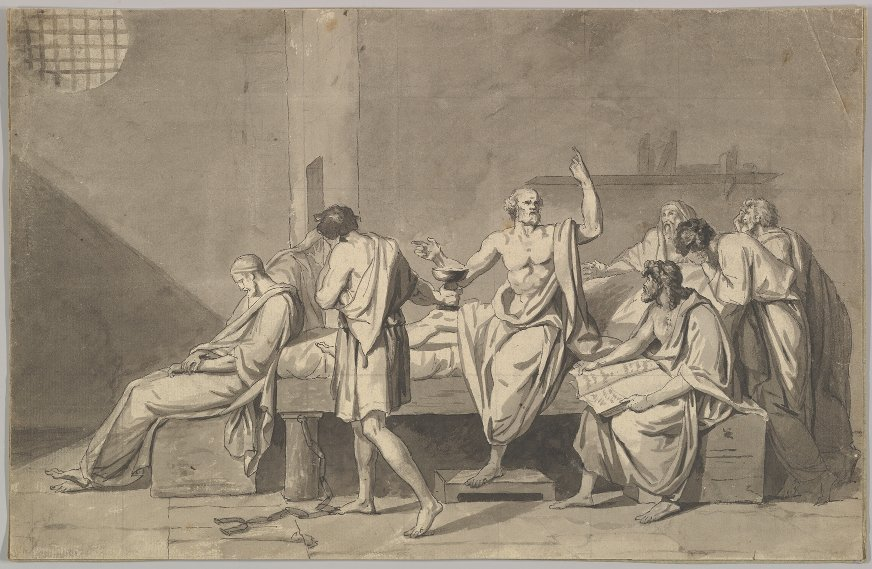
\includegraphics[width=0.5\textwidth,height=\textheight]{img/david-socrates.jpg}

\begin{centercap}

Jacques-Louis David, ``The Death of Socrates''

\end{centercap}

\end{centerpic}

\begin{epigraph}

The unexamined life is not worth living.\\
~\\
---Socrates

\end{epigraph}

\textbf{\emph{Human beings}} have a unique capacity, the ability to reflect on what we believe and do. Unlike other animals, we can take a distance from the evidence of our senses and ask ourselves, ``Should I trust what I see or not?'' Likewise with desire and action: we can examine our own desires, intentions and plans and ask ourselves, ``Should I act on these or not?'' In both cases we are capable of stepping back from the immediate demands of our situation and seeking orientation from another source -- we seek \emph{reasons} to believe or doubt what we see and \emph{reasons} to follow or resist our urges. This reflective capacity is the source of our strength since it has enabled us to both understand and manipulate the world around us like no other creature on the planet. But it also puts us in the uniquely awkward position of having to justify ourselves to our own worst critics, ourselves.

\textbf{\emph{Shakespeare's tragic figure}} of Hamlet sums this up well when he proclaims,

\begin{quote}
What a piece of work is a man! how noble in reason! how infinite in faculties! in form and moving how express and admirable! in action how like an angel! in apprehension how like a god! the beauty of the world, the paragon of animals! And yet to me what is this quintessence of dust?
\end{quote}

\textbf{\emph{The capacity}} to reflect is the source of both our godlike ``apprehension'' and the difficulties we inevitably encounter in figuring out what we should do. Even though, thankfully, most of us do not experience the tension between these two aspects of our ability to reflect on ourselves and our circumstances quite as dramatically as Hamlet did, all of us face this essentially human predicament. As we will be seeing in this text, philosophical ethics is another, much less bloody, way of exploring this predicament. To set the stage for what we will be up to here I want to first say a bit more about our unique reflective capacity and our ability to pay attention to reasons. Then I'll turn to a more detailed account of what is distinctive about philosophy in general and philosophical ethics in particular.

\hypertarget{what-do-i-know}{%
\section{What do I know?}\label{what-do-i-know}}

\textbf{\emph{To start out}} I don't want to exaggerate too much our differences from the other organisms with which we share the planet, since we do have quite a bit with in common with them. We may be, as Aristotle's definition of human beings has it, ``rational animals,'' but we are still animals, and like all other animals with nervous systems we can do two things. We can perceive what is happening around us and we can respond in real time. Animal nervous systems are the product of hundreds of millions of years of evolution, and are extremely useful for helping animals survive and flourish in a complex and constantly changing environment. What is distinctive about the human nervous system is the degree to which the constant stream of information coming into it through our senses is integrated and organized. It is integrated in an experience which is, as far as we can tell, more fully conscious than that of other creatures. And it is organized more explicitly, as is especially evident in our ability to use language.

\textbf{\emph{And likewise}} with the equally constant stream of information produced by our nervous systems, which controls our bodily and verbal responses and the way these both in turn feed back on our thought processes. That these are capable of being integrated and organized in ways that are unique to humans is clearly demonstrated in the astonishing variety and complexity of human cultural and social forms. Of course animals out-perform humans in a variety of specialized tasks, but human achievements in the worlds of culture and society are seemingly capable of infinite variation and complexity ranging from Simone Biles to the internet, from the modern corporation to Tuvan throat singing.

\textbf{\emph{Above all}} it is our capacity for language use that makes possible the integration and organizational flexibility of the human mind. As just one example of how this works, our ability to use and understand language enables us to explicitly categorize and classify what we experience -- things are not just there in our surroundings as objects we happen to come across. Instead we both consciously and unconsciously organize the things we encounter into groups based on concepts such as: edible or inedible, animate or inanimate, threatening or safe, members of our social group or not members of our group, male or female, cause or effect, and so on. Now although there is clear evidence that many animals do this as well -- dogs, for example, distinguish between their owners and strangers, vervet monkeys make different alarm calls for different predators -- for us, these acts of categorizing and classifying can be endlessly expanded and modified and also made explicit to our own awareness. We can endlessly expand our categories to include anything and everything conceivable - ``80's hair bands,'' ``things not good for eating in bed,'' ``mops,'' and ``former presidents,'' just to give a quick random sample.

\textbf{\emph{Not only do we}} thus have an infinitely variable way of looking at the world and organizing our experience according to concepts and categories, but we can see and understand how we are doing so by reflecting on it and talking about it. We can make it explicit how our experience of things is organized and maybe even do it in a different way. We can add new categories or modify how we use them as we notice new similarities or subtle distinctions among things. We may also revise and refine our categories as accumulated personal and shared experience reveals to us their strengths and weaknesses -- whether they ``carve nature at its joints'' or not. This ability to look at things in new ways as a result of collectively accumulated experience is rooted in the fact that we use language to do so and language is both infinitely extensible and essentially shared with other humans. Most importantly for the story I am telling here, we can ask ourselves about the implications of the way we look at the world, and we can wonder about whether we \emph{really} have good reasons for looking at things as we do.

\textbf{\emph{This is a point}} that it is hard to overemphasize but also easy to miss since we take it so much for granted. By asking ourselves about the reasons we have for believing that some aspect or other of our experience is true we are asking ourselves not only about the way things are, but about the way things \emph{should} be; not just what we happen to believe about things based on their appearance to us, but about what we \emph{should} believe about them because it reflects their true reality. And by asking ourselves such questions we are asking what philosophers call normative questions, questions that have to do with values, with concepts like right, wrong, good, bad, true, false, beautiful and ugly.

\hypertarget{what-should-i-do}{%
\section{What should I do?}\label{what-should-i-do}}

\textbf{\emph{Thus far}} I have been emphasizing the role of reflection and the seeking of reasons in our attempts to understand the world in which we live. But this of course is an incomplete picture, since we are not just disembodied minds looking at and trying to figure out the world. We are embodied, social beings who feel and act on needs and impulses, experience emotions, form and try to realize intentions, coordinate or compete with others, and seek or shun each others' company. This practical side of human life is equally capable of being made explicit and becoming an object of our reflective awareness. We don't have to simply act on whatever urges we feel most strongly, we can stop and think about what to do instead. And maybe we can choose to do things differently based on what seems to us to be a better \emph{reason} to act.

\textbf{\emph{Once again}}, just as in the case of belief, our ability to reflect on our choices and actions introduces a normative dimension to human life as we come to ask ourselves questions about our own needs, desires and decisions. We may wonder what we \emph{should do} in some particular situation, perhaps when our feelings are telling us one thing and our experience is reminding us of the bad results the last time we acted on similar impulses. And this generalizes as well -- as we come to reflect on our motivations as such, on which of our goals are more worth pursuing in the long run, on the nature of human motivation and goals in general, and on what might truly be the best way to live our lives. And thus philosophical ethics is born as a product of reflection on our own decision making as potentially thoughtful social animals.

\textbf{\emph{To see how this plays out}} and what a philosophical approach to decision making might look like consider the following dilemma.

\hypertarget{a-difficult-case}{%
\subsection*{A difficult case}\label{a-difficult-case}}


\begin{rmdquestion}

Imagine that you are standing next to a railway track and notice a runaway trolley coming down the tracks. There are five children further down the track who are too far away to hear you. There is also a switch in front of you, that would divert the trolley to the other track. Unfortunately there is also a single worker on the other track, who is himself to far away to hear you.\\
~\\
\emph{Would you throw the switch and cause the worker to most likely die in order to prevent the runaway trolley from hitting the children?}

\end{rmdquestion}

\textbf{\emph{This classic case}} of an ethical dilemma has been extensively studied by philosophers and moral psychologists.\footnote{Originally developed by Judith Jarvis Thompson 50 years ago, this problem has lately seen practical application in the development of self-driving cars., Lauren Cassani Davis, ``Would You Pull the Trolley Switch? Does It Matter?'' The Atlantic, 2015, \url{https://www.theatlantic.com/technology/archive/2015/10/trolley-problem-history-psychology-morality-driverless-cars/409732/}} It presents us with a situation in which we most likely feel torn between two alternatives, neither of which seems to be acceptable or desirable, but in which we also may feel unable to refuse to pick either. Cases like this are good at bringing to the surface the intuitions and assumptions we make about what the right thing to do might be, and that is why they are often studied by philosophers and others interested in looking more closely at moral decision making. One significant result of the study of this case is that a large majority of people say that if they were in that situation they \emph{would} throw the switch. That is, many of us find compelling a common moral intuition that might be expressed by the rule: all else being equal, do whatever saves the most lives. Consider, however, the following variation on this case.

\begin{rmdquestion}

Imagine that you are standing on a bridge with a low railing over a railway track and notice a runaway trolley coming down the tracks. There are five children further down the track who are too far away to hear you. There is also a very large person standing next to you, and if you gave him a slight push he would fall in front of the trolley car causing it to derail, thus saving the five children.\\
~\\
\emph{Would you push the person off of the bridge in order to prevent the runaway trolley from hitting the children?}

\end{rmdquestion}

\textbf{\emph{In this case}} a large majority of people say they \emph{would not} push the person off of the bridge even if it would save the five children. Given that the result is the same in either case, the question then becomes why it is that in the this version of this scenario we no longer look at it in terms of the intuition that it is better to do what leads to more lives being saved.

\textbf{\emph{Whatever the explanation}} for this discrepancy may be (and there is an entire academic industry that has developed around research into the trolley dilemma) the important point here is that philosophers are interested in both examining cases like this directly and in studying how it is that we all tend to respond. Cases like this help us to see and hence to start examining the deeper assumptions we rely on in our thinking about right and wrong. In general this is what philosophy as a discipline is all about -- exposing to view and carefully examining the assumptions we make about how the world works, what we can know about it, and what matters. This is exactly what Socrates meant by leading ``an examined life.'' He insisted that if we never bothered to reflect on our own deepest assumptions about reality, knowledge and values we would be missing out on what make truly makes life worth living. You may disagree with him that this kind of examination is something that we should all devote our entire lives to as he did, but he does have a point worth considering. If we never take the time to deeply reflect on our assumptions, are really ever living \emph{our own} lives?

\hypertarget{philosophical-ethics}{%
\section{Philosophical Ethics}\label{philosophical-ethics}}

\textbf{\emph{Philosophical ethics}} is nothing but the deliberate pursuit and clarification of this kind of reflection on our own values, actions and decisions. Even though, as I have been emphasizing, we all have the capacity to reflect on our lives and choices, we do not always spend the time or make the effort to do this carefully and deeply. This is because we are mostly preoccupied with the immediately practical details of our lives. We are too busy living to take the time to stop and think about the significance of what we are doing. However, at times in the lives of both individuals and societies the need to reflect more clearly on what we are doing becomes more of an imperative. For individuals the need to stop and think and to reconsider the basic assumptions on which we act often arises in relation to important life events or radical changes -- the sudden loss of a loved one; the birth of a child; living through a natural disaster or a war; or even the transition to adulthood in which one assumes full moral and legal responsibility while also gaining the full rights and privileges of adults. These are topics and situations, as we will see later, that are often the focus of discussions in the branch of philosophical ethics called applied ethics. In the case of societies, philosophical thinking likewise flourishes in times of great stress or change -- for example when radically different societies suddenly make contact with each other; when new groups and ways of living displace old groups and ways; when new discoveries challenge peoples' basic views of the nature of things; when societies find their very existence threatened by seemingly insurmountable obstacles. In cases like these it becomes more obviously important to reflect carefully on what we assume is of value to us individually and as a society, on what counts as a good life.

\textbf{\emph{A philosophical approach}} to ethics, or moral philosophy\footnote{Throughout this book I'll be using the terms ``ethics'' and ``morality'' as basically synonymous. Some people distinguish between the two terms in one way or another and that is fine as far as it goes. But since the reason English has both terms is that we borrowed each from a different language -- ``ethics'' comes from Greek, while ``morality'' comes from Latin -- and both original terms mean something pretty similar, I see no reason to insist on any fundamental different meaning between them.}, is concerned with a number of different kinds of questions. Thus the broader field of ethics can be divided up into a number of different sub-fields. These are:

\hypertarget{descriptive-ethics}{%
\subsection*{Descriptive ethics}\label{descriptive-ethics}}


\begin{rmdquestion}

\begin{itemize}
\tightlist
\item
  What do people really think about right and wrong?
\item
  How can we best describe and explain people's moral claims and beliefs?
\end{itemize}

\end{rmdquestion}

\textbf{\emph{Descriptive ethics}} is not exclusively a philosophical approach to ethics in that sociologists, psychologists, anthropologists and other social scientists may also be concerned with people's ethical beliefs. This approach looks at our beliefs about ethical issues and about ethics in general as facts about us to be cataloged and explained.

\hypertarget{meta-ethics}{%
\subsection*{Meta-ethics}\label{meta-ethics}}


\begin{rmdquestion}

\begin{itemize}
\tightlist
\item
  How does thinking about ethics work?
\item
  What are the differences between ethical claims and claims about the facts?
\end{itemize}

\end{rmdquestion}

\textbf{\emph{Meta-ethics}} is a higher-order or ``meta-level'' discussion \emph{about} ethical thinking. Here again, philosophers as well as social scientists often ask meta-ethical questions in their attempts to understand what is distinctive about ethical thinking as opposed to other modes of cognition. But looking at ethics from this perspective does not involve taking a stand on particular ethical principles or issues.

\hypertarget{prescriptive-ethics}{%
\subsection*{Prescriptive ethics}\label{prescriptive-ethics}}


\begin{rmdquestion}

\begin{itemize}
\tightlist
\item
  What is really the right thing to do?
\item
  What moral principles are really justified and should be followed?
\end{itemize}

\end{rmdquestion}

\textbf{\emph{This approach}} to ethics is the uniquely philosophical attempt to find the true basis of ethical thinking. We will be spending a lot of time here examining various attempts to give an account of the basis and justification of ethical thought, belief and action. This way of approaching ethics is not scientific, to the extent that science concerns itself with ``value-neutral'' descriptions and explanations of whatever phenomena it is addressing. That philosophy can succeed in making normative claims while remaining based on objectivity and rationality is up to philosophers to establish.

\hypertarget{applied-ethics}{%
\subsection*{Applied ethics}\label{applied-ethics}}


\begin{rmdquestion}

\begin{itemize}
\tightlist
\item
  What is the right thing to do in real-world cases of ethical controversy?
\item
  What assumptions and principles lie at the basis of ethical controversies?
\end{itemize}

\end{rmdquestion}

\textbf{\emph{How does all of this play out}} in real life cases? Under this heading are also to be found discussions of ethical issues associated with some particular area of human life, profession, or subject matter -- hence medical ethics, business ethics, legal ethics, environmental ethics, bioethics and so on are sub-fields within applied ethics.

\textbf{\emph{We should keep in mind}} as we proceed that these various approaches are not always so clearly separate from one another. Our description of what people believe about ethical questions, for example, is clearly often informed by what we think they are justified in believing. Nevertheless we should keep in mind the fact that we can look at ethics from each of these different points of view and recognize that failing to do so may result in unnecessary confusion.

\textbf{\emph{In conclusion}} we might say that philosophical ethics involves deliberately reflecting on our ideas about ethics in general and on specific applications of these ideas to actual cases and controversies. Another term for such deliberate reflection is ``critical thinking.'' This should not be looked at as a primarily negative activity as the word ``critical'' might suggest, but as the positive attempt to arrive at the truth of the matter by thinking carefully about what are often complex and ambiguous ideas and concepts. Even though, as I mentioned at the outset, all of us are equally capable of reflecting critically on our own beliefs, desires, actions and values, it does take some effort and quite a bit of practice to be able to do so effectively. This is because critical thinking is a skill like anything else that we might do with our minds (like solve algebra problems or identifying different species of trees) and we shouldn't expect to be experts at it from the start. In the \protect\hyperlink{logic}{next chapter} we will look at and get some practice using one of the most important tools for critical thinking -- the logical analysis of arguments.

\hypertarget{further-exploration}{%
\section*{Further exploration}\label{further-exploration}}


\begin{itemize}
\item
  For a slideshow that summarizes the points covered in this chapter, \href{https://gwmatthews.github.io/ethics-slideshows/01-introduction.html}{click here}.
\item
  Michael Sandel is a philosophy professor at Harvard who teaches a very popular course called ``Justice'' that explores material that overlaps with this text. His extensive website \href{http://justiceharvard.org/}{Justice with Michael Sandel} also has videos of his lectures from that course the first of which focuses on the famous runaway trolley example.
\end{itemize}

\hypertarget{logic}{%
\chapter{A Little Bit of Logic}\label{logic}}

\begin{centerpic}

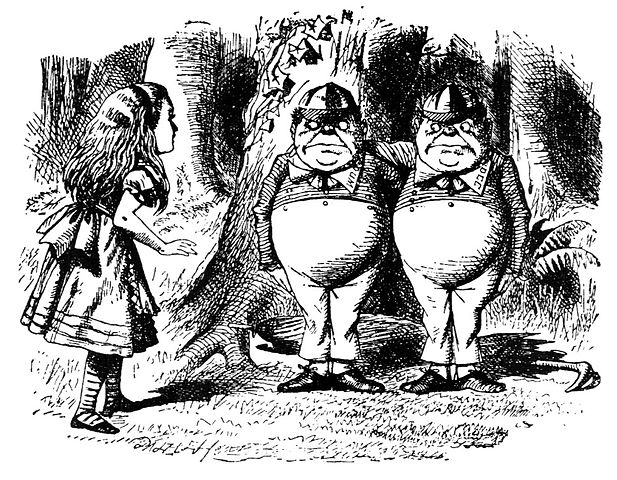
\includegraphics[width=0.5\textwidth,height=\textheight]{img/tenniel-tweedle-dee-dum.jpg}

\begin{centercap}

John Tenniel, ``Alice meets Tweedle Dee and Tweedle Dum''

\end{centercap}

\end{centerpic}

\begin{epigraph}

`Contrariwise,' continued Tweedledee, `if it was so, it might be; and if it were so, it would be; but as it isn't, it ain't. That's logic.'\\
~\\
---Lewis Carroll, Through the Looking Glass

\end{epigraph}

\textbf{\emph{Logic}} is the formal study of reasoning -- the attempt to justify or provide evidence for claims or beliefs. In this chapter we will look at the basic concepts and techniques for the logical analysis of arguments. As we will be seeing this will be useful in our discussions of ethics since much of what we will be doing will involve careful consideration of the justification of claims we make about ethics in general as well as particular topics in ethics.

\textbf{\emph{Before}} we get started though we need to clarify some terminology -- especially our use of the word ``argument.'' Too often this word conjures up a pointless verbal fight between people with opposed views. They argue rather than discuss because their differences of opinion are fixed in place and neither will budge. It is typically a good idea to stay away from arguments in this sense. The word argument as we are using it here, however, has quite a different meaning. For us arguments do not require differences of opinion because arguments are just attempts to explicitly provide back-up or justification for some claim that we might make. We offer arguments in this sense whenever we make the grounds for our belief explicit whether we are doing this within the confines of our own heads, in written form or spoken out loud whether or not anyone disagrees with us. Arguments in this sense of the term might appear in regular old verbal disputes. But as we will be seeing arguments are best looked at one at a time since each one stands or falls on its own merits.

\textbf{\emph{So, for philosophers,}} arguments are just attempts to provide support for whatever it is that we might claim is true. For example, maybe we think the death penalty is wrong, or the opposite, so we come up with an argument to show this. Or maybe we think that morality is a sham, nothing but a cover story for basically selfish motives. Once again, we can come up with an argument in support of this idea. Or on an even more abstract level we might think that moral judgments are just matters of opinion and that it is therefore a waste of time to even argue about what is right and what is wrong. Since none of these claims are self-evidently true (even though some people may think some of these are obvious) we'll need an argument to back it up, or at least to make explicit our reasons for claiming it. In the end, we can think whatever we want. That will, however, only get us so far -- either others will agree with us or not, and either it will be true or not. But we can also offer reasons in support of our claims in the form of arguments. As we will be seeing, not all arguments are equally persuasive, but there are clear cut and reliable ways of evaluating them to see which really provide the support we are after and which do not.

\hypertarget{arguments-rationality-and-rhetoric}{%
\section{Arguments, Rationality and Rhetoric}\label{arguments-rationality-and-rhetoric}}

\textbf{\emph{Arguments}} can of course be looked at as attempts to persuade other people that they should accept the claims that we are making. Because of this it may seem at first glance to be similar to rhetoric, also known as ``the art of persuasion.'' People who study and practice rhetoric often claim that rational argument is just one among many different methods of persuasion, appropriate at specific times, but not fundamentally different than other methods. That is, they claim that argument is a form of rhetoric. Philosophers, on the other hand, would like to insist on the basic difference between the two. Philosophers call attention to the fact that in rhetoric:

\begin{itemize}
\item
  Appeal is made to our emotions, prejudices, fears, hopes, etc. That is, who we are and what we feel about things matters. This is both its strength and its weakness.
\item
  Because of this, the persuasion that rhetoric produces doesn't last, once our feelings change, we are no longer convinced, and our feelings are constantly changing.
\end{itemize}

In rational argument, on the other hand:

\begin{itemize}
\item
  Appeal is made not to our emotions but to our ability to reason.
\item
  Since everyone is equally capable of reasoning, this means that arguments do not appeal to us personally. It doesn't matter who you are, a good argument should convince you.
\end{itemize}

\hypertarget{the-structure-of-arguments}{%
\section{The Structure of Arguments}\label{the-structure-of-arguments}}

\textbf{\emph{To see}} all of this more clearly, we need to take a look at how arguments work. But first things first -- we need a more precise definition of what we mean by an argument in the first place. That's easy enough:

\begin{rmdnote}

An argument is a series of statements where some of these statements are intended to provide evidence or support for others. When we argue we are attempting to establish some claims on the basis of other claims.

\end{rmdnote}

\textbf{\emph{As sets of statements}}, arguments involve the declarative use of language. Declarative statements (or propositions) are just sentences that state stuff, they make claims, and so they can be either true or false. So when we are looking at arguments we are deliberately ignoring the many other ways we can use language, such as asking questions, making commands, expressing feelings. When we are offering an argument we are making a series of claims in which some are supposed to provide support for others. The statements that are doing the supporting are known as \emph{premises}. The statement that is being supported, the point of our argument is called the \emph{conclusion}.

\textbf{\emph{It is, however,}} sometimes difficult to tell whether a set of sentences is an argument or not. Let us consider a few examples:

\begin{center}

\begin{argument}

Parents should have the right to make decisions about their own children's healthcare.\\
Why should other people mess around in their business?\\
And please, let's keep the lawyers out!

\end{argument}

\end{center}

This may seem like an argument, so how can we tell for sure? Simply by checking whether this set of sentences is a set of statements where some are intended to provide support for others. So, how many statements are there here? Only one: the first sentence is a statement, the second is a question and the third is a command. In other words, even though this looks at first like an argument it is really just a single claim with no real argument given in support.

\textbf{\emph{What about}} the next example? How many statements are in these sentences? And do any of them really offer support for any of the others?

\begin{center}

\begin{argument}

I am convinced that aliens are living among us and you should be convinced as well.\\
I have really good evidence for this claim.

\end{argument}

\end{center}

Well this is almost an argument, but not quite. There is a claim being made here: aliens are living among us. But there is no real support given for this claim, only the insistence that this person has some unknown evidence. Before we can start to evaluate this evidence to see whether it really supports the claim, we need to see it. So here we have only two separate statements without a real argument yet.

\textbf{\emph{Now consider}} the following example:

\begin{center}

\begin{argument}

Christopher Columbus was a criminal, because anyone who kills innocent people, kidnaps others, and steals their valuables is a criminal and that is just what he did.

\end{argument}

\end{center}

Here the grammatical form is a little misleading. This is an argument in spite of the fact that there is only one sentence. Why? Because this one sentence expresses a few different claims or propositions and some of these claims are offered as supports for others. We can see this if we break it up into individual claims and change the order around like so into \textbf{standard form} with the premises listed as individual statements and the conclusion written last.

\begin{center}

\begin{argument}

Anyone who kills people, kidnaps other people and steals their valuables is a criminal.\\
Christopher Columbus did all of those things.\\

So Christopher Columbus was a criminal.

\end{argument}

\end{center}

Perhaps this is not yet a very convincing or complete argument, but at least it is an argument unlike the first examples.

\textbf{\emph{It is not}} always so clear which statements in an argument are the premises and which statement is the conclusion. Often, but not always, these are signaled with one of a number of typical words or phrases that function as premise or conclusion indicators. Paying attention to these typical words and phrases can help you to disentangle the argument from the peculiarities of a writer's style.

\hypertarget{premises}{%
\subsection*{Premises}\label{premises}}


\textbf{\emph{To help guide}} us through an argument a writer or speaker who is presenting an argument might use the following expressions and phrases to show what the argument rests on. These are \emph{premise indicators}.

\begin{rmdnote}

\begin{itemize}
\tightlist
\item
  Because
\item
  Since
\item
  In light of the fact that
\item
  In view of the following evidence
\end{itemize}

\end{rmdnote}

This is not an exhaustive list. Basically, when reading an argument you can pick out the premises by asking yourself where the writer is starting from and where he or she is going. The first is the set of premises and the second is the conclusion.

\hypertarget{conclusions}{%
\subsection*{Conclusions}\label{conclusions}}


\textbf{\emph{It is often}} the case that arguments are presented with the conclusion first in order to emphasize where the discussion is supposed to be going. The following common words are often used to indicate a statement that is supposed to play the logical role of the conclusion of an argument.

\begin{rmdnote}

\begin{itemize}
\tightlist
\item
  Therefore
\item
  It follows that
\item
  Thus
\item
  It should be clear that
\end{itemize}

\end{rmdnote}

These words and phrases indicate that this is where the writer (or speaker) is going with the argument and they are often used at the beginning of an informal argument to orient us, even though logically speaking they are last. For example, when a lawyer begins her argument in court with the claim, ``Your honor, ladies and gentlemen of the jury, my client is not guilty,'' and then goes on to present the evidence, she is reversing the logical order for rhetorical effect. This is fine in everyday life, but since it can be confusing, when we look at arguments explicitly here we will look at them in standard form with the premises first and conclusion last.

\hypertarget{pattern-of-reasoning}{%
\subsection*{Pattern of reasoning}\label{pattern-of-reasoning}}


\textbf{\emph{One other thing}} to watch for when looking at arguments is words and phrases that indicate the structure of the reasoning itself. These are ways of pointing out exactly how the premises are supposed to support the conclusion, and so are indicators of the pattern or form of reasoning involved. Some examples are:

\begin{rmdnote}

\begin{itemize}
\tightlist
\item
  Because of these, that has to be true.
\item
  If this then that, otherwise this.
\item
  All of the above is true so this means\ldots{}
\item
  This is the only option that makes sense.
\item
  If we assume that this is true we get a ridiculous result so it can't be true.
\end{itemize}

\end{rmdnote}

These indicate the general logic form of argument being followed. Is it a matter of necessity, other conditions present or absent, summation of influences, or a process of elimination, or are we showing something indirectly by showing that denying it makes no sense? The more formal study of logic looks carefully at these and many other different patterns of reasoning, and we will meet them at various points in our discussions of arguments about topics in ethics.

\hypertarget{validity-and-soundness}{%
\section{Validity and Soundness}\label{validity-and-soundness}}

\textbf{\emph{Not all arguments}}, however, are really equal. Just having any old argument won't always get us very far. Instead, as we will see, there are some arguments that really are better than others. This was the insight of the first philosophers in the Western tradition, Socrates, Plato and Aristotle, and it does seem kind of strange that I feel compelled to have to justify it even after a couple of thousand years. Way back then, just like now, many people thought this was a presumptuous claim to make. This is especially the case since it amounts to the claim that some arguments are really compelling on their own, and that we should, as long as we are being rational, have no choice but to accept them. For the skeptics out there who doubt that we will ever be able to create such an argument, I should also point out that the clearest and best arguments really don't end up saying anything very controversial or extraordinary. This is one of the limitations that logic imposes on us: if we are really being logical and using only reliable arguments we may have to refrain from claiming to be able to establish very much. Understanding the logic of arguments, if nothing else, should encourage us to be a little more modest in our claims to knowledge. And this is why Socrates, in spite of his reputation for being a bit of a jerk in pointing out to many people the flaws in their own arguments is today most well known for saying that the only thing he really knew what how little he knew.

\textbf{\emph{To get back to business,}} when we are arguing what we are doing is trying to establish the truth of something that we don't know on the basis of other things that we already know or accept. What we are interested in is establishing the truth of the conclusion, yet for some reason it's truth is not obviously apparent to us so we need to establish it on the basis of other claims the truth of which we can already accept. Arguments move us from the known to the unknown.

\textbf{\emph{To take}} a simple example, suppose we would like to establish that Socrates fears death. We don't have any direct reason for thinking that this is true. But we do know some other things that may be of use in establishing this. First we know that Socrates is a human being. Second we know that all human beings are mortal. Third, we know that all mortals fear death. In standard form this would be arranged like so:

\begin{center}

\begin{argument}

Socrates is a human being.\\
All human beings are mortal.\\
All mortals fear death.\\

So Socrates fears death.

\end{argument}

\end{center}

This is a bit of a contrived example, but it can help us to see the key concepts we can use to evaluate any argument at all.

\hypertarget{key-concepts}{%
\subsection*{Key concepts}\label{key-concepts}}


\textbf{\emph{The information}} in the premises is enough information, as we can easily see, to establish our conclusion. Since Socrates is human he must be mortal, and he must fear death, since all mortals fear death. This argument seems like a pretty solid piece of reasoning. But how can we tell in general whether an argument is a good argument? It turns out that there are two questions we will need to ask about an argument in order to determine whether or not it is a good argument:

\begin{rmdnote}

\begin{itemize}
\tightlist
\item
  Is there a clear and solid connection between every step of the reasoning that leads us inevitably from premises to conclusion? In philosophical terminology: \textbf{is it valid}?\\
  ~\\
\item
  Are the claims that we started from, our premises, really true? In philosophical terminology: \textbf{is it sound}?
\end{itemize}

\end{rmdnote}

How do we answer these questions for the example above? It seems that there is in fact a clear and solid connection between what the premises are saying and what the conclusion is saying. In fact we already showed this above when showed that the conclusion necessarily follows from the premises. Technically this is a short and informal \emph{proof} of its strength as an argument, that is, of its validity. So the answer to the first question is, yes, it is valid.

\textbf{\emph{As far as}} the second question goes, however, we may have our doubts. Are all of the premises really true? Socrates is (or was) a human being -- he was one of the first philosophers. And all human beings are in fact mortal, at least as far as the evidence we have goes. But do we really know whether all mortals, past, present and future fear death? So here is the one small weakness of the argument. If we could be assured that this premise was true the argument would be completely convincing and would provide adequate backup for the conclusion. But it rests, unfortunately, on a weak premise, so it is not a sound argument. Since these two ideas are both very important for everything we'll be doing here and not so obviously obvious, here are some more explicit definitions:

\begin{rmdcaution}

The best arguments must be both \emph{valid} and \emph{sound.}

\begin{itemize}
\item
  \textbf{Validity}: in a valid argument IF the premises are true the conclusion MUST also be true.
\item
  \textbf{Soundness}: A sound argument is a valid argument that also has TRUE premises.
\end{itemize}

\end{rmdcaution}

One thing to notice here is that the test for validity is entirely independent of the test for soundness. It is a little misleading, as we can now see, to ask whether arguments are either good or bad. More precisely, they can be:

\begin{itemize}
\item
  \emph{Valid and sound}: these are the best arguments, because the premises really establish the conclusion, and the premises are true -- hence the conclusion really is true.
\item
  \emph{Valid but not sound}: these are promising arguments that exhibit good logical form, but that rely on less than perfect information in their premises, and so are not completely solid.
\item
  \emph{Invalid}: these arguments are bad arguments since they do not establish what they claim to be establishing. All invalid arguments are automatically unsound, since sound arguments are a subset of valid arguments.
\end{itemize}

\hypertarget{more-examples}{%
\subsection*{More examples}\label{more-examples}}


\textbf{\emph{Learning how}} to identify valid arguments is important for a course in philosophical ethics, since the philosophical approach to ethics consists largely of the examination of arguments about ethical issues. And the best way to learn this is by practicing. Consider the following argument, conveniently written in standard form:

\begin{center}

\begin{argument}

The earth is a rotating sphere moving around the sun.\\
We are all on the surface of the earth.\\
Anything on the surface of a moving object moves with that object.\\

So we are all moving around the sun.

\end{argument}

\end{center}

Forget for a moment about whether or not you buy the conclusion on its own. In analyzing an argument we need to know whether the premises support the conclusion adequately, so we pretend that we are not sure about the truth of the conclusion. Our first test is the test of validity. We ask ourselves: if the premises were true, could the conclusion be otherwise? Is the truth of the conclusion guaranteed by the truth of the premises? In this case it seems clear that if we are in fact all on the surface of an object that is moving around the sun, then we would all also have to be moving around the sun. So the argument is valid.

\textbf{\emph{Notice}} that establishing an argument's validity is not yet establishing that the conclusion is really true. It is only establishing that the conclusion would be true, if only we could show that the premises were true. In fact this argument was rejected until about 500 years ago because nobody was willing to accept the truth of the first premise. Establishing that this was true took quite a bit of effort by Copernicus, Kepler, Galileo and other early modern scientists. However, we now know that the premises are true. So this argument is not only valid, but also sound. And since it is sound we have proven beyond the shadow of a doubt that the conclusion is true. One more thing to point out here is that this argument has always been sound (or at least as long as the solar system has existed) even if many people denied the truth of the first premise. They were simply mistaken in this denial.

Let's look at another example:

\begin{center}

\begin{argument}

If you want to see the world, you should join the navy.\\
Jane wants to see the world.\\

So Jane should join the navy.

\end{argument}

\end{center}

This argument is a little trickier because it contains an \emph{If \ldots{} then} statement. If \ldots{} then statements, also known as conditionals, make indirect claims. They don't just tell us what is the case, they tell us what would be the case if, or on condition that, something else were true. With this in mind let us consider this second argument. First we check for validity, by assuming that the premises are true and seeing if the conclusion would have to be true as well. In other words we are not yet interested in whether or not they really are true, but whether the argument works as an argument, whether the conclusion logically follows from the premises. It seems pretty clear that this argument is valid. This is because \emph{if}, as the first premise claims, the navy really is the best way to see the world, \emph{and if} as the second premise claims, a person named Jane wants to see the world, then she should clearly join the navy. Notice that this argument's validity does not have anything to do with its content, with the particular claims being made. Instead, validity is a matter of form, so that we could substitute any other content for the content of this argument without affecting its validity. Essentially this argument has the following form:

\begin{center}

\begin{argument}

If A, then B.\\
A.\\

Therefore B.

\end{argument}

\end{center}

\textbf{\emph{Here}} A, B can be substituted by any statements we please, as long as our substitution is consistent throughout the argument. In all cases the resulting argument will turn out to be valid. Try it and you will see that the resulting arguments all come out valid. This is because validity is a matter of logical form regardless of the content we are arguing about.

\textbf{\emph{The soundness}} of arguments, however, unlike validity, has everything to do with content, because an argument is sound when it is valid and it \emph{also has true premises}. Back to the argument about Jane. Is it sound? First we note that it is valid, then we ask whether or not the premises are really true. Consider the first premise: ``If you want to see the world you should join the navy.'' It may be true that joining the navy is one way to see the world (provided that you don't end up on a submarine, or in the engine room of a ship), but is it the only way? Of course not, so the first premise is just false. The second premise is also questionable, but for a different reason -- we simply do not know who Jane is since this is a fictional example. So in spite of its validity this argument is unsound and we need not accept the conclusion as a true statement. It may in fact be true, but this argument gives us no good reason for thinking so. As an exercise you might want to try coming up with a sound argument that follows the form of this one.

\textbf{\emph{Now consider}} as our next example, the following argument:

\begin{center}

\begin{argument}

If you want to see the world, you should join the navy.\\
Jane joined the navy.\\

So Jane wants to see the world.

\end{argument}

\end{center}

This argument seems similar to the previous one, but it has one important difference. The conclusion of this argument was the second premise of the last argument, and the second premise of this argument was its conclusion. What happens to the validity of the argument when we make this simple change? Notice what this argument is saying. It is offering an explanation of why it is that Jane joined the navy -- because she wanted to see the world. The question is, and this is the way we check for validity, are there any other possible explanations of why she joined the navy that are consistent with the premises? In other words, \emph{is it possible for the premises to both be true and the conclusion false}? The answer is yes. It all hinges on what the first premise doesn't say. It doesn't say that the only possible reason to join the navy is the desire to see the world. It just says that if that's what you happen to want then the navy is for you. So Jane could have joined the navy only because she wanted to learn all there is to know about marine diesel engines without caring whether she learned this in New Jersey or in the South Pacific ocean. To put this in yet another way: if it is at all possible, if there are no contradictions involved, for the premises of an argument to be true and the conclusion false, then the argument is invalid. This argument is invalid for precisely this reason. Furthermore, since it is invalid, this automatically makes it unsound, since in order for it to be sound it has to first be valid.

\hypertarget{proofs-and-counterexamples}{%
\section{Proofs and Counterexamples}\label{proofs-and-counterexamples}}

\textbf{\emph{Another}} way to look at the difference between valid and invalid arguments is in terms of the difference between a proof and a counterexample. A proof is a step by step demonstration that the conclusion is a \textbf{necessary} consequence of the premises. To prove that a conclusion validly follows from a set of premises we show in a detailed way how a series of obviously valid steps in reasoning lead us to the conclusion. Take the following argument for example.

\begin{center}

\begin{argument}

Fred is older than Wilma but younger than Betty.\\
Barney is older than Betty.\\

So Barney is older than Fred.

\end{argument}

\end{center}

Remember that a valid argument is one in which \textbf{\emph{if}} the premises are true, the conclusion must also be true. So how would we prove that this is the case? Well we just \emph{assume} that the premises are true and go from there. So here is what a proof might look like:

\begin{rmdtip}

The first premise states that Fred is older than Wilma and he is younger than Betty. Wilma doesn't matter here since she isn't mentioned in the other premise or the conclusion, so let's just note that this premise clearly states that Fred is younger than Betty. Now this would mean that Betty is older than Fred, since ``older'' and ``younger'' are inverses. If I am younger than you then you are older than me no matter who we are since that's what ``younger'' and ``older'' mean. Now since Barney is older than Betty, as the second premise states, he must be older than Fred too, since as we just saw, Betty is older than Fred. This follows from the fact that the relationship ``older than'' is a \textbf{transitive} relationship -- if A is older than B and B is older than C A has to be older than C since that's ``just what''older than" means. So our conclusion that Barney is older than Fred is clearly a \emph{logical consequence} of the premises.

\end{rmdtip}

\textbf{\emph{That's all}} there really is to any proof. We have just unpacked the meaning of what the premises are saying in a way that establishes that they entail the conclusion. We don't, in other words, have to add any new information to what is already stated in the premises in order to get the conclusion. In more complicated cases it can take much more effort to show this but all proofs are nothing but such a process of showing that the conclusion is thus ``contained'' in the premises already, which is of course \emph{why} the truth of the premises would guarantee the truth of the conclusion. In a simple case like this we can almost just see the obviousness of the connection between premises and conclusion, and so it might seem silly to spell things out in this much detail, but in more complicated cases there is more room for error so spelling things out like this is important.

\textbf{\emph{Invalid arguments}} in contrast are arguments where we would need something more than what is contained in the premises to get the conclusion. No matter how we attempt to prove our conclusion we will \emph{always} come to some spot where we cannot get any closer to the conclusion. So how do we show \emph{this}? We use a counterexample, which is nothing but a possible situation in which the premises would all be true and the conclusion would be false. This shows that the argument is invalid, since if it were valid it would be \emph{impossible} for the premises to be true and the conclusion false at the same time as we just saw. Consider the following argument:

\begin{center}

\begin{argument}

Fred is older than Wilma but younger than Betty.\\
Barney is younger than Betty and older than Wilma.\\

So Fred is older than Barney.

\end{argument}

\end{center}

Even though we have no idea what these peoples' ages are (or even if they exist outside of a 1970's TV cartoon series) we can tell that the conclusion does not have to be true, even if the premises were true. This argument is invalid and we can show this with a counterexample.

\begin{longtable}[]{@{}cc@{}}
\toprule
person & age\tabularnewline
\midrule
\endhead
Barney & 36\tabularnewline
Betty & 40\tabularnewline
Fred & 35\tabularnewline
Wilma & 32\tabularnewline
\bottomrule
\end{longtable}

\textbf{\emph{Notice that}} if these people had these ages, this would make all of the premises true and the conclusion false. If Fred is 35, Wilma is 32, Betty is 40 and Barney is 36, then it is true that Fred is older than Wilma, but younger than Betty -- which is what the first premise claims. It is also true that, given these ages, Barney is younger than Betty and older than Wilma -- which is what the second premise claims. But Fred is not older than Barney. In other words, what these ages show that it is \emph{possible} for the premises to be true and for the conclusion to be false and thus that the reasoning involved in getting to the conclusion is invalid. Even if we had true premises, this would not be enough to guarantee the truth of the conclusion. That is what terrible reasoning is all about. We will many more examples of bad reasoning in the next chapter on logical fallacies.

\hypertarget{further-exploration-1}{%
\section*{Further exploration}\label{further-exploration-1}}


\begin{itemize}
\item
  For the slideshow summarizing the main points of this chapter, \href{https://gwmatthews.github.io/ethics-slideshows/02-logic.html}{click here}.
\item
  For a slightly different and more in-depth treatment of the basic concepts of logic see \href{https://jonathanweisberg.org/vip/logic.html\#logic}{the logic chapter} of Jonathan Weisberg's open source textbook on probability and statistics, \emph{Odds \& Ends.}
\item
  Wireless Philosophy is a well-produced series of short videos on a great many topics in philosophy. Their \href{https://www.youtube.com/playlist?list=PLtKNX4SfKpzX_bhh4LOEWEGy3pkLmFDmk}{playlist on Logic and Critical Thinking} is a great resource for exploring logical thinking in all of its complexity, 5 or 6 minutes at a time.
\end{itemize}

\hypertarget{fallacies-and-biases}{%
\chapter{Fallacies and Biases}\label{fallacies-and-biases}}

\begin{centerpic}


\includegraphics[width=0.4\textwidth,height=\textheight]{img/illusion.png}

\begin{centercap}

\href{https://pixabay.com/users/openclipart-vectors-30363/}{OpenClipart-Vectors} at pixabay.com

\end{centercap}

\end{centerpic}

\begin{epigraph}

Reality is, you know, the tip of an iceberg of irrationality that we've managed to drag ourselves up onto for a few panting moments before we slip back into the sea of the unreal.\\
~\\
---Terence McKenna

\end{epigraph}

\textbf{\emph{Throughout}} our discussions of logic so far, you may all have been wondering how often anyone ever lives up to the standards of logical reasoning as we have laid them out here. It may seem fairly obvious that most people do not seem to be either willing or able to accept only those claims that are conclusions of sound arguments, but instead we often decide based on feelings and instincts or on the basis of what we just want or assume to be true at the outset. In fact, there is a theory of the origins of our capacity for logical reasoning known as the ``\href{https://www.edge.org/conversation/hugo_mercier-the-argumentative-theory}{argumentative theory of reasoning}'' that claims that our logical abilities, such as they are, evolved to enable us to ``prove'' ourselves right. Before the abstract study of logic was invented by Aristotle, who sought the universal principles governing reasoning, we were all already adept at persuading others by manipulating logic for the sake of convincing others that we were right and hence asserting social dominance, whether or not our claims were truly justified. It seems, in other words, that the rhetoricians were right after all that logic is just one means of persuasion among others, no better or worse than them, but maybe more or less effective in different contexts.

\textbf{\emph{Or is it?}} As we saw in the last chapter, there is something to be said for being logical. Put simply, valid and sound reasoning really just boils down to not saying more than you really know and this seems like a pretty reasonable approach if we want to figure out what is true and what is not. It is, however, abundantly clear that us humans often fail to abide by this principle and make claims that we really don't have much support for. This chapter explores two related ways we do this -- by committing fallacies and by getting caught by various ``cognitive illusions.'' Fallacies are bad arguments -- they are typically invalid -- that are often used to try to convince someone of some point that really has little argumentative support. They work, to the extent that they do, because they take advantage of certain weaknesses in our reasoning skills. As we will be seeing, a careful analysis of how various different forms of fallacious reasoning work and of what mistakes they make can provide us with a certain degree of protection from those who would use them to convince us of things that have little real support. Cognitive illusions are related in that they lead to mistakes in reasoning, but they are often more difficult to spot and avoid falling prey to, since they are mistakes rooted in mental shortcuts that can be reliable in certain contexts. Like visual illusions, they are false representations of reality, which, even if we know they are false, we cannot help falling prey to. Looking at some common cognitive illusions can help us to see, however, why we should sometimes not trust our own thought processes as much as we often do. And this as well can provide us with more tools for distinguishing between between what is really the case and what just seems to be so.

\textbf{\emph{As we turn to examine}} some important logical fallacies it is helpful to keep in mind that there are both many more particular fallacies than the ones we are going to look at and also many different ways of categorizing them. The thing to keep in mind here is that all stretch logical support beyond its breaking point, and how in particular this happens is not always so clear. On the other hand you can usually see the weakness of an argument that relies on a fallacy by asking yourself a simple question about it: What is being claimed here, and on the basis of what? This often reveals the basic weakness of the argument as it involves stepping back from the particular claims being made in order to see the broader pattern and strategy of reasoning involved. It is this pattern that is flawed, regardless of the content of the argument. As a result, we can often find instances of the same form of fallacious reasoning used with many different topics, especially those that are controversial.

\textbf{\emph{In addition}} it can be helpful to look at fallacies in terms of a few more general types of mistakes in reasoning. That is what we will do here as we examine some different forms of bad reasoning under the headings: \protect\hyperlink{relevance}{fallacies of \emph{relevance}} all of which depend on premises not relevant to the conclusion; \protect\hyperlink{ambiguity}{fallacies of \emph{ambiguity}} all of which depend on the ways in which many words and expressions can have multiple and often incompatible meanings; and \protect\hyperlink{presumption}{fallacies of \emph{presumption}}," which depend on unacknowledged, unjustified extra assumptions.

\hypertarget{relevance}{%
\section{Fallacies of Relevance}\label{relevance}}

\textbf{\emph{As we turn to}} the fallacies of relevance, it is good to remember these fallacies depend on the use of information that may seem relevant to establishing the conclusion but isn't really relevant after all. They often play on our emotional responses to certain situations and topics and they can be quite effective as means of persuading us. They work so well in getting us to buy into their conclusions in part because of the nature of the human mind -- even though we are capable of thinking about things coolly and logically, we often jump to conclusions on emotional grounds and then enlist our cognitive abilities merely to rationalize decisions and conclusions we have already made. Philosophers would encourage us to resist such impulses and to stop and think before jumping to conclusions. This can of course be quite challenging just because of the way in which our brains are wired -- the neural pathway between sensory input to motor and cognitive output is shorter in its trip through those parts of the brain that process emotions than it is through our higher cognitive powers. But still, whoever said leading an examined life was the easiest thing to do?

\hypertarget{appeal-to-authority}{%
\subsection*{Appeal to authority}\label{appeal-to-authority}}


\begin{center}

\begin{argument}

My friend who is a scientist insists that global warming is not cause for alarm, and for me that is a good enough reason to accept her conclusion.

\end{argument}

\end{center}

\textbf{\emph{This fallacy}} is also known as ``appeal to inappropriate authority.'' Appealing to authority is a commonly used way of trying to convince people. But why do we find authorities believable in the first place? Because they are authorities? In this case we may wonder why they are considered authorities at all. On the other hand if they have something to back up their claims, why don't we just see for ourselves whether they are right or not?

\hypertarget{ad-hominem}{%
\subsection*{Ad hominem}\label{ad-hominem}}


\begin{center}

\begin{argument}

There is no need to take that animal rights activist seriously.\\

After all, she also benefits from the use of animals -- notice her leather shoes and fur mittens.

\end{argument}

\end{center}

\textbf{\emph{The name}} of this fallacy is a Latin expression meaning ``against the person.'' It is also known as the ``abusive fallacy,'' or ``personal attack.'' This very popular fallacy focuses on the personal inconsistency of the person giving the argument in an attempt to discredit their argument. People who use this strategy don't respond directly to their opponent's argument but bring up external reasons not to believe anything he or she says. This is clearly wrong since it is the argument that someone gives and its validity and soundness that should be our concern not the person from whose mouth that argument happens to be coming.

\hypertarget{popular-appeal-bandwagon-fallacy}{%
\subsection*{Popular appeal (bandwagon fallacy)}\label{popular-appeal-bandwagon-fallacy}}


\begin{center}

\begin{argument}

The Romans were justified in slaughtering thousands of slaves.\\

After all it was a part of their culture and not many people objected.

\end{argument}

\end{center}

\textbf{\emph{This fallacy}} involves appealing to what most people or the majority of people think as a way of determining what is really true or really right. But as pre-civil rights segregation laws show -- what the majority wants or believes can very easily be wrong. The fallacy known as the ``appeal to tradition'' is similar in that it claims that tradition, the way people have been doing things for a long time, is a good enough basis for us to believe or act as they did. This, of course overlooks the possibility that they were wrong or had no good reason to believe or act as they did.

\hypertarget{appeal-to-force}{%
\subsection*{Appeal to force}\label{appeal-to-force}}


\begin{center}

\begin{argument}

The reason that we are right is because we have the military might to get rid of any government that disagrees.

\end{argument}

\end{center}

\textbf{\emph{However effective}} force or threats of force may be in getting people to do what we want, we may wonder whether this approach really is attempting to convince anyone of anything. Even though threats may get people to say that they agree with you, this shows nothing about whether or not the conclusion is true or whether they really believe what you are saying.

\hypertarget{appeal-to-consequences}{%
\subsection*{Appeal to consequences}\label{appeal-to-consequences}}


\begin{center}

\begin{argument}

If astronomers are correct, the earth orbits a relatively insignificant star in a remote corner of one galaxy among billions.\\

But this conclusion violates our sense of the significance of our own lives and so it must be false.

\end{argument}

\end{center}

\textbf{\emph{This fallacy}} involves rejecting some particular viewpoint, theory or idea based on the consequences to which it leads. These consequences are often emotionally loaded, the kinds of things that we may not want to believe. However, it is often simply irrelevant whether or not we like or want to believe something: the truth may in fact be indifferent to what is pleasing to us. The way to tell what the truth of the matter is, is to examine the evidence rather than reject a theory out of hand because it has unappealing consequences.

\hypertarget{the-naturalistic-fallacy}{%
\subsection*{The naturalistic fallacy}\label{the-naturalistic-fallacy}}


\begin{center}

\begin{argument}

Women alone are capable of having babies.\\

So the responsibility of raising and taking care of them is entirely theirs.

\end{argument}

\end{center}

\textbf{\emph{Next we have}} the naturalistic fallacy. We often appeal to nature as if natural things, practices, etc. were automatically good. This is perhaps understandable in a world filled with various artificial substances of dubious safety. But we should be careful of making such appeals since they involve a leap of logic. The problem with the naturalistic fallacy is actually quite a general problem -- the attempt to conclude something about what should or ought to be be the case from what simply is the case. In this example, the facts of how human reproduction work entail nothing about who should play what role in raising children. That is a matter of social relations that, us philosophers hope, should be based on a free and open (and rational) discussion between those involved and not on the ``facts of life.''

\hypertarget{the-genetic-fallacy}{%
\subsection*{The genetic fallacy}\label{the-genetic-fallacy}}


\begin{center}

\begin{argument}

Newspapers are businesses that make profits from selling papers.\\

So we should distrust what they publish since it is bound to be affected by their desire to make money.

\end{argument}

\end{center}

\textbf{\emph{Arguing like this}} is a more general version of the naturalistic fallacy. We often assume that where something comes from affects its nature in fundamental ways and so we automatically tend to distrust research that is paid for by corporations, we distrust claims made by people who stand to gain from what these claims are about and so on. Although it may seem like wise advice to ``follow the money'' and keep in mind that those who pay the bills might use their power to determine the content of the conversation, insisting that \emph{this must be} the case simply does not follow. In the case of the news media, the fact that a large newspaper corporation makes money for its employees doesn't automatically slant what exactly they are saying in one way or another. This is because one part of their business strategy might also be to maintain high standards of independently verified journalistic integrity. If they are selling their repuation as reliable reporters, and there is an independent way f=of determining the truth of their claims, there is not necessarily a conflict built into the idea of selling newspapers. Just as in the case of other fallacies of relevance, such as appeak to authority and ad hominem, in this case waht matters is not so much who is saying something but what is being said, and we can see for ourselves whether or not it is reliable or slanted in any way.

\hypertarget{red-herring}{%
\subsection*{Red herring}\label{red-herring}}


\begin{center}

\begin{argument}

We shouldn't worry that much about people dying of horrible diseases in Africa.\\

After all we have problems of our own to deal with.

\end{argument}

\end{center}

\textbf{\emph{The name}} of this fallacy comes from the British method of fox hunting. First a captive fox is released and then a pack of foxhounds follow its scent trail, followed in turn by the hunters. In order to make it a little more difficult for the hounds to follow the fox, a piece of smoked herring (a smelly fish that typically is red in color) is wiped on the ground across the fox's path and thrown off to the side somewhere. This serves to distract and confuse the hounds and gives the fox a chance to get away. In an argument whenever you bring up something irrelevant in order to draw attention away from the topic at hand you are relying on the fallacy of red herring. The problem with the reasoning in this example, of course, is that there is no mention made of the possibility that both problems in Africa and problems here can be addressed. Besides mentioning something off the topic in no way undermines whatever claims are made about that topic.

\hypertarget{weak-analogy}{%
\subsection*{Weak analogy}\label{weak-analogy}}


\begin{center}

\begin{argument}

Galileo was ridiculed because of his views, and these views later proved to be correct.\\
I too am ridiculed for believing that the Pope is a reptilian alien in league with the Freemasons.\\

Thus I too will have my day and my views will be accepted.

\end{argument}

\end{center}

\textbf{\emph{Analogies are}} comparisons between different things. We reason analogically when we argue that because one object or concept has a certain feature, other objects or concepts that are similar in certain respects will also have that feature. This is an important way in which we make sense of the world. However, it has its drawbacks. If we are not careful we can end up making analogies when they are not really there. This argument is based on a weak analogy because it is just not the case that all views that are ridiculed end up prevailing in the end. Some do, like Galileo's, but the reason was not inherent in their being ridiculed, but on their being based on good reasoning supported by evidence in the appropriate ways. And by the way, there really are people who believe that the Pope is a reptilian alien, just google it and see.

\hypertarget{ambiguity}{%
\section{Fallacies of Ambiguity}\label{ambiguity}}

\textbf{\emph{The next set}} of fallacies relies on the fact that many terms have multiple meanings. Switching between meanings without acknowledging that one is doing so is a way of making invalid reasoning look valid. Closer examination reveals arguments that do this to be weaker than at first glance. Here we will consider just a few examples. Many more often appear in debates and you can find out about many more examples by following the links at \protect\hyperlink{further-3}{the end of this chapter}.

\hypertarget{equivocation}{%
\subsection*{Equivocation}\label{equivocation}}


\begin{center}

\begin{argument}

People in jail are really free.\\

This is because if you can think whatever you want, then you are free and people jail can certainly think whatever they want.

\end{argument}

\end{center}

\textbf{\emph{Equivocation}} is using multiple meanings of a word as if they were the same. We start out with one meaning of a word like ``freedom'' and end up with another meaning, in the attempt to fool the person who is listening to us that our reasoning is valid. Since many words have multiple meanings it is important to watch out for subtle shifts as an argument progresses.

\hypertarget{straw-person}{%
\subsection*{Straw person}\label{straw-person}}


\begin{center}

\begin{argument}

The senator who suggested cutting funding for the new Air Force attack drone system really wants to leave us defenseless against our enemies.\\

Thus we should reject such cuts.

\end{argument}

\end{center}

\textbf{\emph{This fallacy}} often appears in the context of a debate in which one person misrepresents his or her opponent's view in order more easily to knock it down, like a person made of straw. This is a fallacy of ambiguity in that it relies on a superficially similar version of the view that is being attacked rather than the view itself. One can often ``win'' debates by using this strategy, but such victories are hollow in that they do not really engage with the real issues. If you really want to demonstrate that some view you are attacking is worthy of rejection, it is far better to rely on the ``principle of charity'' and present your opponent's view in as favorable a light as possible. If it still fails, then your position may look even better. The drawback, however, is that if you represent your opponent's views in a more fair and favorable light, your objections to them may themselves not hold up. But that is really only a drawback if you care more about winning debates rather than in figuring things out.

\hypertarget{cherry-picking}{%
\subsection*{Cherry picking}\label{cherry-picking}}


\begin{center}

\begin{argument}

This study of 12 children clearly shows a link between childhood vaccination and autism.\\

Thus vaccines cause autism.

\end{argument}

\end{center}

\textbf{\emph{This one}} is really no joke -- in fact the whole of the current scare about childhood vaccinations and autism was ``established'' by a single study of twelve children! The fact that the paper was retracted, and its author was barred from medical practice didn't matter since its influence only grew since the date of its publication. The logical mistake here is that of selectively reading the evidence in favor of your own hypothesis, or ``cherry picking'' the data to get the juiciest bits while ignoring anything that contradicts it. The other name for this fallacy, ``Texas sharpshooter'' refers to the related practice of proving your worth as a target shooter by first shooting random holes in the side of a barn, and then afterwards drawing your target around a cluster of holes so that it looks like you are a great shot. Is this done in Texas? Probably not, but whoever named it must have had a low opinion of Texans -- no offense intended and if you are from Texas, substitute your state of choice.

\hypertarget{presumption}{%
\section{Fallacies of Presumption}\label{presumption}}

\textbf{\emph{The third set}} of fallacies we will consider here are those that make presumptions, often in a hidden way. That is, they rely on hidden and unstated assumptions written, as it were, between the lines. This strategy, however, cannot withstand critical analysis since if we can get the perpetrator of such fallacies to acknowledge these hidden presumptions we can see them for what they are, mere assumptions without warrant.

\hypertarget{mere-assertion}{%
\subsection*{Mere assertion}\label{mere-assertion}}


\begin{center}

\begin{argument}

Abortion is just wrong, and that is all there is to it.

\end{argument}

\end{center}

\textbf{\emph{This is}} the simplest and most obvious kind of bad reasoning. As the name implies, mere assertion involves simply stating what you want to establish without presenting any evidence whatsoever to support it. It is truly amazing how often people simply assert something that they may think is true without bothering to offer anything to support this assertion.

\hypertarget{begging-the-question}{%
\subsection*{Begging the question}\label{begging-the-question}}


\begin{center}

\begin{argument}

You should become a Christian.\\
This is because the Bible says that if you are not a Christian you will go to Hell.

\end{argument}

\end{center}

\textbf{\emph{This strange sounding}} name really applies to a very simple technique. Someone who begs the question is guilty of assuming what they are claiming to establish in their argument. In other words they put a disguised version of their conclusion in the premises of their argument. That is, they are not really arguing for what they claim to be arguing for. This is an example of a fallacy that is nevertheless a valid form of reasoning. The problem here is that we cannot just assume that the conclusion is true, as someone who uses this way of argument is in fact doing. Begging the question is not, of course, always so obvious. We can see that this is a case of begging the question when we realize that the only people who will be convinced by this argument are Christians. Why? Simply because nobody else will take evidence from the Bible seriously, and people who consider the Bible as authoritative are already Christians. This example also shows why begging the question is also known as ``preaching to those already converted.''

\hypertarget{appeal-to-ignorance}{%
\subsection*{Appeal to ignorance}\label{appeal-to-ignorance}}


\begin{center}

\begin{argument}

The claim that the death penalty deters crime has not been established with any certainty.\\
Thus it is clear that it does not deter crime.

\end{argument}

\end{center}

\textbf{\emph{The fact that}} something has not yet been proven to be true does not mean that it is false. It is just unknown! Yet this fallacy assumes that if we do not have proof of something then that thing must be false.

\hypertarget{false-dilemma-black-or-white-fallacy}{%
\subsection*{False dilemma (black or white fallacy)}\label{false-dilemma-black-or-white-fallacy}}


\begin{center}

\begin{argument}

Either living organisms are products of blind chance or they were deliberately designed.\\
But it makes no sense that something as functionally complex as a living organism is the result of blind chance.\\

Hence they must have been designed.

\end{argument}

\end{center}

\textbf{\emph{The argument here}} rests entirely on an assumption that is not always so easy to see, the assumption that the alternatives stated are the only ones there are. If this were the case, then the argument would stand, but often other alternatives are simply not even mentioned. Hence the dilemma, or forced choice between two alternatives, is here a false one. In the example below, which is often used against the theory of biological evolution, the missing alternative is precisely what Darwin articulated in his book \emph{On the Origin of Species}, a theory which contains an element of chance but which is not reducible to the blind chance that this argument presumes is the only alternative to deliberate design.

\hypertarget{hasty-generalization}{%
\subsection*{Hasty generalization}\label{hasty-generalization}}


\begin{center}

\begin{argument}

All three of my ex-wives always told me what to do.\\

This clearly shows that all women want to control us men all the time.

\end{argument}

\end{center}

\textbf{\emph{We may be tempted}} to conclude a lot from a single case, or a relatively small sample, but this is often merely a way to confirm our prejudices. If we really want to make sweeping generalizations, we'll have to gather a bit more evidence in less clearly biased ways than this.

\hypertarget{slippery-slope}{%
\subsection*{Slippery slope}\label{slippery-slope}}


\begin{center}

\begin{argument}

If we legalize physician assisted suicide then everyone over sixty had better watch their backs.\\

Once doctors get used to helping people with terminal illnesses die comfortably, they'll find it easier to get rid of older people.

\end{argument}

\end{center}

\textbf{\emph{Slippery slope arguments}} are often used as a way of warning us of the dangers of allowing people to do something that is now forbidden. They say, in effect, if we allow someone to do this, then they'll have no reason not to do that, which is much worse. The name comes from the metaphor of an icy ski slope: if we are foolish enough to step onto the slope, without skis on of course, we'll end up uncontrollably sliding down to the bottom. The problem with this argument is that it claims that we must end up where the arguer claims we will, but the argument gives does nothing but assert that.

\hypertarget{false-cause}{%
\subsection*{False cause}\label{false-cause}}


\begin{center}

\begin{argument}

The majority of heroin users smoked marijuana when they were younger.\\
So smoking marijuana must be one of the causes of heroin use.

\end{argument}

\end{center}

\textbf{\emph{Us humans}} are very good at noticing patterns in the world around us. In fact science is based on this ability -- we notice regularities and then come up with explanations for them. The most powerful of these explanations involve attributing a causal relationship between events that appear to be related to each other in a regular way. We have to be careful here, however, since we also have the tendency to overdo this. This may seem like a convincing argument until we recognize that the fact that something tends to happen before something else is not nearly enough to establish that the first thing causes the second to happen. For example, the fact that my alarm clock goes off every day shortly before sunrise does not mean that my alarm clock causes the sun to rise. The same goes for drug abuse. The fact that I abused marijuana first and then heroin later does not mean that the first caused the second. It is equally possible that I abuse whatever drugs I abuse for another reason -- I have major problems I am trying to escape from.

\hypertarget{circular-reasoning}{%
\subsection*{Circular reasoning}\label{circular-reasoning}}


\begin{center}

\begin{argument}

He must be guilty, since he has a guilty look on his face.\\

Furthermore, the look on his face indicates guilt, because he is the one who did it.

\end{argument}

\end{center}

\textbf{\emph{This final fallacy}} in our list is, in a sense, a more complex version of begging the question. Circular reasoning involves bouncing back and forth between two assumptions each of which is supposed to be the basis for the other. To see the circular structure of the reasoning exhibited here it may help to figure out which statement is the premise and which is the conclusion. In this example, at first glance it seems like the conclusion is ``He is guilty,'' and this seems to be based on the premise that ``He has a guilty look on his face.'' However, the fact that the look on his face indicates guilt is then supported by the assertion that ``He did it.'' Clearly we are moving around in a circle -- our premise supports and is supported by our conclusion. There is thus no real support for either and the whole structure is unfounded. This fallacy is also known as the ``vicious circle'' fallacy.

\hypertarget{cognitive-biases}{%
\section{Cognitive Biases}\label{cognitive-biases}}

\textbf{\emph{Fallacies}}, as we have been seeing, are common mistakes that we make in reasoning especially when we are trying to support a conclusion that we have insufficient evidence to support, ways in which we claim more than we really know. In recent years cognitive psychologists have also explored the ways in which not only get our arguments wrong, but also tend to get things wrong in our own thinking, how as Thomas Gilovich puts it in the title of his book \emph{How We Know What Isn't So}.\footnote{Thomas Gilovich, \emph{How We Know What Isn't So} (New York: The Free Press, 1991)} That is, we have a tendency to fall prey to biases and mistakes in our own reasoning whatever it is that we may end up defending later in our arguments. In this section we'll look at some of the most important and relevant of these cognitive biases.

\textbf{\emph{In general}} we might classify these biases into two general types: ``hot biases,'' or motivated irrationality where our interests, emotional responses or visceral reactions to things influences our thinking process; and ``cold biases'' or unmotivated irrationality which are a result of certain mental shortcuts and routines we rely on even in situations where they do not really apply. Let's look at some examples.

\hypertarget{hot-biases}{%
\subsection*{\texorpdfstring{\textbf{Hot Biases}}{Hot Biases}}\label{hot-biases}}


\textbf{\emph{Hot biases}} are also known as examples of ``motivated irrationality'' because they involve bending our reasoning to suit our wants and desires. Our motivations may not always be clear even to us, so we may not realize that we are caught up in such biases. Luckily, however, there are steps we can take to avoid falling prey to them.

\hypertarget{confirmation-bias}{%
\subsection*{Confirmation bias}\label{confirmation-bias}}


\textbf{\emph{Confirmation bias}} is our often unconscious tendency to give more weight to evidence supporting our pre-existing beliefs or hypotheses and our tendency to downplay the significance of evidence against them. The result is similar to cherry picking but it may not be a deliberate attempt to mislead, but more of a product of other unconscious tendencies.

\begin{center}

\begin{argument}

I keep seeing more and more evidence in favor of my hypothesis! What about the evidence against it? Well that must be based on faulty data collection.

\end{argument}

\end{center}

Given that we have a strong tendency to fall prey to this bias, what steps might we take to avoid it? For one, we can use various ``blind'' methods of data collection and analysis to protect our reasoning from the errors involving confirmation bias. ``Double blind'' medical trials follow these precautions -- to avoid confirmation bias, the patients involved in the trial of a new drug, for example, don't know whether they are getting the drug or a pacebo, and the researchers also don't know whether each particular patient they examine afterwards are in the test group who receive dthe drug of the control group that didn't

\hypertarget{group-think}{%
\subsection*{Group think}\label{group-think}}


\textbf{\emph{Just like}} our pre-existing beliefs can influence what we take the evidence to support, likewise with our connections to other people can do so. When someone in a group we identify with comes up with an idea we have tendency to give it more weight than in fact it deserves. A great example of this occurred during the Kennedy administration with the Bay of Pigs incident. The plan was to send a small group of armed anti-Castro Cuban soldiers to the Bay of Pigs in Cuba with the thought that that would be enough to incite a full-scale revolt against the Communist government by the rest of the Cuban population. Enough members of Kennedy's National Security Council which planned and approved the incursion were strongly in favor of it that they collectively ignored their own military intelligence which indicated that there was little popular support for revolting against the Cuban government. So when the invasion happened in January 1961 the initiative was quickly defeated and the Cuban exiles who landed in the beach were quickly arrested and imprisoned much to the embarrassment of the Kennedy Administration.\footnote{``Bay of Pigs - Groupthink,'' accessed December 2, 2019, \url{https://www.globalsecurity.org/intell/ops/bay-of-pigs-groupthink.htm}}

\hypertarget{wishful-thinking}{%
\subsection*{Wishful thinking}\label{wishful-thinking}}


\textbf{\emph{These last two}} biases could be considered specific examples of a more general tendency we have towards wishful thinking, which is the tendency to project our own desires onto reality and fool ourselves into thinking that reality conforms to how we would like it to be.

\begin{center}

\begin{argument}

I just know that the Yankees will win the World Series, they just can't let me down again!

\end{argument}

\end{center}

All of these biases fail to make a distinction between what we would like to be the case and what really is in fact the case. We may end up lucky and happen to find out that reality conforms to how we would like it to be, but then again we may not. We can protect ourselves against these kinds of biases first by being aware of our own tendencies to fall prey to them and then by using particular strategies to separate our analysis of the evidence from our wishes.

\hypertarget{cold-biases}{%
\subsection*{\texorpdfstring{\textbf{Cold biases}}{Cold biases}}\label{cold-biases}}


\textbf{\emph{Cold biases}} differ from hot biases in that they are not such much results of our desires but of the ways in which our cognitive systems work. They are more like ``bugs'' in our mental operating systems than ways in which we twist our thoughts to conform to our desires.

\hypertarget{anchoringframing-effects}{%
\subsection*{Anchoring/framing effects}\label{anchoringframing-effects}}


\textbf{How much} are you willing to pay for some given product or service? Well it turns out to depend not just on the features of that product or service itself but also by what is next to it on the shelf, what other options you are presented with and even the initial asking price. These are examples of the ways in which the context of our choices influences the content of our choices. Many examples of this can be found in the marketplace. The notorious ``bait and switch'' tactic relies on this bias.

\begin{center}

\begin{argument}

Today only, you can get a new Toyota for 20\% off the sticker price! So act now and drive your new car away today!

\end{argument}

\end{center}

There are numerous ways in which advertisers and salespeople try to influence our choices. First the ``sticker price'' may or may not reflect anything about the reality of the product in question but may be intentionally inflated to anchor our minds to a price higher than we would actually pay. It turns out that doing so will make us more willing to pay a higher price than we would if the original non-discounted price were set closer to what we might actually pay, or what the manufacturer expects us to pay. Likewise, adding extra options that we may not actually be interested in independently can influence our willingness to buy a product, especially when it is compared to an otherwise equivalent product without those potions. In both cases our ability to compare what is offered with what we want is corrupted by the context within which the product is presented.\footnote{For more on anchoring effects see Daniel Kahneman, \emph{Thinking Fast and Slow} (New York: Farrar, Straus and Giroux, 2011)}

\hypertarget{the-fundamental-attribution-error}{%
\subsection*{The fundamental attribution error}\label{the-fundamental-attribution-error}}


\textbf{\emph{When it comes to}} explaining human behavior, and trying to figure out the relative weights of internal factors such as needs, desires and the personality of the actor on the one hand, and external situational factors on the other hand it turns out that we come up with different weights when thinking about our own behavior and that of other people. our own and others. We tend, for example, to put more weight on things outside of our own control when accounting for our bad behavior than we do when accounting for the behavior of others.

\begin{center}

\begin{argument}

The fact that I tripped when walking down the street was because the sidewalk was uneven. When you trip on the other hand, it's evidence that you are a klutz.

\end{argument}

\end{center}

\textbf{\emph{In other words}} we are more generous with ourselves in terms of getting ourselves off the hook --- it's not my fault it's the situation I was in --- than we are with others --- clearly it is their fault! This is true that in many, many cases, if we looked at things in the more neutral terms of finding what factor most influence all of our behavior situational or external factors often play a much greater role than we think. So we are more accurate when we reflect on ourselves than when we look at the behavior of other people. Our attribution of causal influences tends to be skewed in the wrong direction when we look at why others do what they do especially when we compare it with our understanding of what influences us ourselves.

\hypertarget{the-availability-heuristic}{%
\subsection*{The availability heuristic}\label{the-availability-heuristic}}


\textbf{\emph{Finally}} in this brief survey of some major cognitive biases we have the confusion we tend to make between how readily something comes to mind (its ``salience'') and the more objective probability of its occurrence (its ``frequency''). Thus because terrorist attacks are so dramatic and stand out in our minds much more than the more common and mundane threats we are exposed to we tend to be more afraid of terrorism than, for example, driving to the airport. In the aftermath of the 9/11 attacks I remember listening to an interview with an expert on national security threats. The interviewer asked him what we could all do to be safer in international air travel and his response was ``Drive very carefully to the airport.'' This effect, once you start to notice it, is everywhere. We focus on dramatic if also highly unlikely threats and events and ignore those that are far more likely and hence, paradoxically, not so obvious to us.

\textbf{\emph{In this}} and the last chapter we have taken a closer look at what is involved in the justification of any claim at all. We have seen that the best arguments are both valid and sound -- they work logically in that their premises really provide adequate support for their conclusions and their premises are actually true. We have also examined some of the many mistakes in reasoning to which we are prone. These mistakes are not only used in a deliberately misleading way, since all of us have a tendency to make decisions and judgments first and then come up with reasons in support of them later. Thus we often rely on fallacious reasoning to rationalize our own beliefs or we tend to read the evidence is biased ways. As we will be seeing, as we turn now to start examining some of the many different theoretical approaches to ethics, the tools of logic and critical thinking will prove very useful in trying to come up with a reasonable answer to the general question, ``what is the right thing to do?''

\hypertarget{further-3}{%
\section*{Further exploration}\label{further-3}}


\begin{itemize}
\tightlist
\item
  Here is a \href{https://gwmatthews.github.io/ethics-slideshows/03-fallacies.html}{summary in slideshow form} of the content of this chapter.
\end{itemize}

\textbf{\emph{There are many}} great websites that list, discuss and explain the many ways we get things wrong in our thinking. Here are a few of my favorites.

\begin{itemize}
\item
  \href{https://yourlogicalfallacyis.com/}{\emph{Your Fallacy Is}} is a nicely designed website with more examples of common fallacies.
\item
  \href{https://yourbias.is/}{\emph{Your Bias Is}} is the sister site to Your Fallacy Is and focuses on common cognitive biases.
\item
  \href{https://www.logicallyfallacious.com/tools/lp/Bo/LogicalFallacies}{\emph{Logically Fallacious}} is a site with a huge and comprehensive list of logical fallacies and cognitive biases. A great reference with lots of examples.
\item
  Dan Ariely is a behavioral economist who studies human irrationality and has written a number of very readable books documenting his findings. He also has a number of videos of talks he has given on his site, \href{http://danariely.com/}{danariely.com}

  \begin{itemize}
  \tightlist
  \item
    \url{http://danariely.com/}
  \end{itemize}
\item
  And you should of course follow the \href{https://twitter.com/fallacy_ref}{Logical Fallacy Ref} on Twitter.
\end{itemize}

\begin{centerpic}

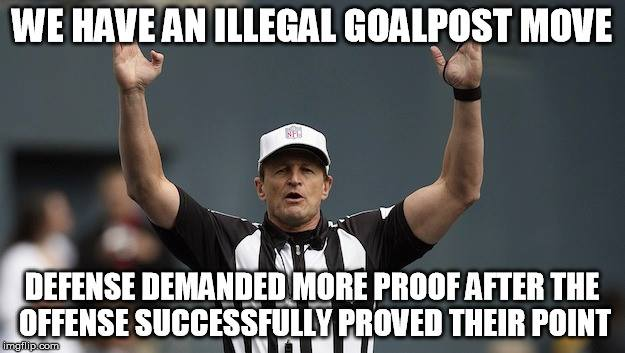
\includegraphics[width=0.5\textwidth,height=\textheight]{img/fallacy-ref.jpg}

\end{centerpic}

\hypertarget{part-ethics-culture-and-religion}{%
\part{Ethics Culture and Religion}\label{part-ethics-culture-and-religion}}

\hypertarget{relativism}{%
\chapter{Relativism}\label{relativism}}

\begin{centerpic}


\includegraphics[width=0.5\textwidth,height=\textheight]{img/buddha-bird.jpg}

\begin{centercap}

\href{https://pixabay.com/users/mikhsan-4911734/}{mikhsan} at pixabay.com

\end{centercap}

\end{centerpic}

\hypertarget{approaching-ethics}{%
\subsection*{Approaching ethics}\label{approaching-ethics}}


\textbf{\emph{As we now turn}} to look more carefully at ethics it may help to have a sense of the general approach we will be following here. We'll be looking at a variety of theoretical perspectives on ethics -- perspectives which determine the position one might take regarding questions such as:

\begin{itemize}
\tightlist
\item
  Is ethics just a matter of opinion, or is can ethical principles lay claim to a more universal validity?
\item
  What is the relation between ethics, law and religion -- all of these spell out rules for behavior but on the basis of what and what happens when they come into conflict?
\item
  Is it rational to be ethical or does ethics depend on something other than our ability to think things through?
\item
  Is there anything that is just plain wrong, no matter what the consequences?
\end{itemize}

\textbf{\emph{There are many possible ways}} to consider these questions. I'll be following a fairly common approach that looks at them in the light of various general theories or philosophical positions one might adopt. Each of these theories makes a particular claim about what is fundamental to ethics, highlights certain aspects of our ethical lives and also provides some guidance for dealing with ethical controversies in the real world. These theories have all found both defenders and critics in the history of philosophy although here I will be more concerned with them as general approaches to ethics than with worrying too much about accurately presenting the views of historical thinkers. These theories as I am presenting them can best be looked at as ``ideal types'' that have their own inner logic, and their own strengths and weaknesses as attempts to articulate and defend some version of what ethics is really all about.

\textbf{\emph{In my view}} not all of these theories are equally viable. In fact it seems to me that most of them simply fail as approaches to ethics for a variety of reasons that will become clearer in each case. This brings up the obvious question of why we should bother looking at a whole slew of approaches to ethics that ultimately don't work instead of just more directly articulating one that does. There are two reasons to take this approach. First, in spite of the difficulties faced by these approaches to ethics, \emph{all} of them continue to be popular and find defenders both historically and at the present. Even if these defenses are inadequate, they still have and have had their champions. There is a version of an old joke about anarchists that applies here to philosophers: given three philosophers in a room together there will be four positions taken by them on any topic that comes up for discussion. This is a feature and not a bug of philosophy, since philosophy is the attempt to articulate and defend a general account of such abstract topics as the nature of reality, knowledge and values, so the more particular positions we can examine the better. Just like in science we should welcome a diversity of approaches rather than rule any out at the start. But unlike in science, unworkable philosophical theories have a longer shelf life since the cost for holding on to them is relatively easy to bear. If a scientific theory is fatally flawed that is typically clear -- one's prediction of what the experiments or data will show fails, other explanations cover more cases with fewer assumptions and better fit with the data, the bridge built on the basis of one's calculations collapses. The cost of bad science is steep. In philosophy, however, the costs of holding onto unsuccessful theories is having to put up with theoretical incoherence, to be willing to hold conflicting views in the mind at the same time. And it turns out that us humans are pretty good at doing these things -- all you have to do to live with a poorly worked out set of fundamental beliefs is stop thinking about them.

\textbf{\emph{The second reason}} for considering a multitude of unsuccessful approaches to ethics here is that each of these approaches does have the advantage of focusing on some important aspect of ethics. To the extent that these theories fail it is because they tend to overemphasize the aspect in question and ignore others. Looking at a variety of approaches can thus help give us a clearer picture of what ethics as a whole is all about, even in the absence of some final master theory that would unify ethics once and for all and win universal assent. It seems to me that there is a certain ``logic'' to the story I'll be telling here, even if it is nothing like a necessary development, a magical dialectical unfolding of the Truth about ethics, but I do present each theory as an effort to take in to account the failings of the proceeding accounts. Making sense of our ethical lives and thinking clearly about ethics is hard, but it seems to me that it is worth the effort. Philosophical ethics may not be an empirical science, and debates in ethics may not ever be resolved, but it is a rich field well worth exploring. My presentation here is intended in the spirit of a guidebook, pointing out certain general features of the landscape, some important landmarks and major hazards to be reckoned with.

\textbf{\emph{So much for}} a general account of what we will be up to here. This section of the text looks at two approaches to ethics that may seem to be diametrically opposed -- cultural relativism and the attempt to show how ethics can and should be based on religion. According to cultural relativism, ethical rules and norms are determined by culture in the sense that there are no absolute and universal rules with an independent warrant, but only particular, culturally determined ways of conducting oneself, none fundamentally better or worse than the others. According to religious approaches to ethics, ethical rules and principles do have an absolute foundation and that foundation is to be found is an authoritative set of religious truths. In spite of their obvious opposition, with relativism denying the existence of ethical absolutes and religious approaches affirming it, in a sense both have something essential in common, which is the idea that ethical rules come to us ``from outside'' and have little to do with human choices. Their opposition lies in whether or not the source of ethical rules varies from place to place or not. Both of these approaches will be found wanting, for roughly parallel reasons. And so the next part of the text, which examines various more purely philosophical approaches to ethics, takes up the question of what ethics might look like if it is something we humans create and not imposed from outside by culture, God or human nature.

\hypertarget{claims-and-consequences-of-moral-relativism}{%
\section{Claims and Consequences of Moral Relativism}\label{claims-and-consequences-of-moral-relativism}}

\begin{epigraph}

If anyone, no matter who, were given the opportunity of choosing from amongst all the nations in the world the set of beliefs which he thought best, he would inevitably -- after careful considerations of their relative merits -- choose that of his own country. Everyone without exception believes his own native customs, and the religion he was brought up in, to be the best.\\
~\\
---Herodotus, The Histories

\end{epigraph}

\textbf{\emph{Opinion}} -- this seems to be where ethics starts and in many people's minds where it ends. You have a right to your opinion about right and wrong and I have a right to mine, so let's just leave it at that. Given what we have been looking at so far, not to mention all of the unread pages still ahead, it is probably already apparent that that is not going to be the whole story about ethics. It is nevertheless a deeply rooted assumption that ethical claims \emph{must be} opinions, since they are clearly \textbf{not} factual claims and that seems to be the only other sort of claim we can possibly be making when we are using language to state things. That this assumption does not in fact hold up to closer inspection is what this chapter is going to argue.

\textbf{\emph{Humans are}} incredibly diverse and in many ways. We are diverse in appearance; we live in many ways in many different environments; we speak many different languages and embrace many different beliefs, practices and norms. People live in almost any conceivable physical environment, from dense tropical jungles, to frozen polar deserts, from small villages with thatched huts to modern industrial cities made of concrete, steel and glass. In addition, our cultural practices and norms reveal perhaps an even greater diversity. Some human cultures place value on devotion to the group at the expense of individual liberty, others emphasize the unique individual while downplaying our relation with others. Some cultures value continuity and tradition while others value innovation and rapid change. Some cultures value constant productive work while others place far more emphasis on living well and enjoying social interaction with others. Some cultures allow men and women to participate equally in all areas of social life, while others have entirely separate spheres for the two sexes. Recognition of this diversity is what has led some philosophers and social scientists to formulate a theory known as ``cultural relativism,'' which takes these casual observations and turns them into an explicit set of claims about the nature of value judgments. This theory is not only a popular theory about the nature of values. It also presents a challenge to the whole enterprise of philosophical ethics since it leads to the view that rational discussion and argument have little role to play in ethical decision making. Ethical decisions, opinions and judgments, according to cultural relativism, are always relative to the cultural environment within which they are made.

\textbf{\emph{Cultural relativism}} is one particular variant of a broader position that holds that moral universals are impossible in principle and that moral judgments are closer to judgments of taste than they are to anything else. Just as with judgments of taste, according to this view, sometimes called ``moral anti-realism'' for its denial that there is any basis in reality for determining what is right and what is wrong, there is little point in arguing about moral issues since they reduce to personal preferences. I won't go into the various versions of this idea here but will focus on the claim that moral values and judgments are essentially rooted in culture. The issues that this view raises, it seems to me at least are broadly the same as those faced by other variants and so dealing with cultural relativism will be enough for our purposes here.

So let us then look more carefully at what cultural relativism claims. It is a \protect\hyperlink{meta-ethics}{meta-ethical} position that boils down to a few simple and seemingly obvious claims:

\begin{rmdnote}

\textbf{According to cultural relativism}

\begin{itemize}
\tightlist
\item
  Ethical or moral claims are not objective in the way factual claims are.
\item
  There is no neutral standard for determining right or wrong.
\item
  All value judgments are relative to our personal or cultural perspective.
\end{itemize}

\end{rmdnote}

\hypertarget{a-first-case-for-relativism}{%
\subsection*{A first case for relativism}\label{a-first-case-for-relativism}}


\textbf{\emph{At first}} this set of claims may seem obviously true. After all, given the diversity of human values and customs, how could there be anything more than relative standards, standards that are only applicable within a given culture? Many people find relativism intuitively appealing and might even offer as a preliminary case for relativism the following points:

\begin{itemize}
\tightlist
\item
  \emph{Cultural diversity}: Human culture has always been extremely diverse. And many people seem to have equally diverse views on what sort of behavior is acceptable. It seems to follow from this that there cannot possibly be any standards for deciding between these views.
\item
  \emph{How we learn about values}: It seems obvious that we learn about values, and come to accept the values that we do because these are the values that are shared by the people who raise us. They are the values of our families and communities.
\item
  \emph{Intolerance}: There have been plenty of cases throughout history in which one group of people firmly believed that their values were not just acceptable for them but absolutely right, and used this as a justification for committing atrocities against other people. Relativists insist that the only way to avoid this kind of intolerance is to accept that there are no ultimate standards.
\end{itemize}

\hypertarget{what-is-at-stake}{%
\subsection*{What is at stake}\label{what-is-at-stake}}


\textbf{\emph{In a moment}} we will consider each of these points in greater detail. Before we do this it will be helpful to spell out what is at stake here. That is, we should consider what would be the case about ethical principles and decision making if cultural relativism were true. Its defenders make much of the positive consequences of this theory, while its opponents emphasize its negative implications. As we consider these consequences of the theory we must remember that whether or not we like where a theory leads us, in terms of its theoretical consequences, cannot itself determine whether the theory itself is correct. Reality does not care whether or not we like it. In the case of relativism at least, the extreme nature of its consequences helps explain why it is such a controversial theory.

\textbf{\emph{Defenders of relativism}} present it as the best way to acknowledge the great variety of human value systems and cultures. If there are no ultimately correct moral principles, then all human cultures become equally valid as ways of life, at least for different groups of people. This seems to encourage tolerance of other ways, a welcome relief after millennia of people intolerantly fighting with each other over their different views. After all, if there are no ultimate standards for right and wrong, we would could never justifiably say, ``Your group is wrong in doing what you do and so we have the right to force you to change your ways.'' On the other hand, a relativist cannot really consistently promote tolerance -- otherwise she would be granting tolerance for other cultural practices the status of a universal value, valid for everyone and this is what relativism says does not exist. So we should really say that relativism really only rules out one possible way of dealing with conflicts: the rational settlement of differences with reference to some kind of universal principles or values. Sometimes differences of opinions might be tolerated by the members of the groups that differ, sometimes one group will attempt to push its values on the other group. Both approaches are consistent with the claims of relativism.

\textbf{\emph{The first}} troubling consequence of relativism is one you may already have suspected: if there are no real standards, standards about right and wrong that are independent of cultural perspectives, it doesn't seem possible to condemn other cultures or individuals for doing awful things. For example, imagine that there is a society that has two major groups of people. One of these groups, who happen to be the majority of the population, decides that the other group doesn't deserve any respect, perhaps even that they are somehow naturally deficient or inferior. As a result they perform painful and often fatal experiments on the minority group, force them to work without pay, and even decide just to kill them off because it makes them feel better about themselves. What would a relativist say about this? It seems that since the relativist is only willing to recognize local or relative standards, she would have to conclude that although she doesn't like it, or that such behavior would never be tolerated in her society, she really can't condemn what this group of people are doing as simply being wrong. Why not? Well, because it seems right to the majority of people in that other society.

\textbf{\emph{Furthermore}}, relativism, if it were true, would require us to reject the idea that we can really make moral progress. Consider voting rights for women and African-Americans. In early American history both groups were denied these rights. Later on, after the Civil war in the case of African-American men and then in the early twentieth century in the case of all women, the Constitution was amended when people recognized that it was wrong to restrict these groups' access to the political process just because of race or gender. Many of us would consider this a case of moral progress -- a basic right was extended to people who had previously, for no good reason, been denied this right. What would a relativist say? Could they say that this was really a case of progress? Probably not, since progress implies that things are getting better, and this requires that there is some standard against which we can measure better or worse. So, for the relativist there is no such thing as progress, only different ways of doing things, none of which are really better or worse than any others. Is this a conclusion you are comfortable with?

\textbf{\emph{Relativism seems}} like a plausible theory about the nature of value judgments. It also seems, at first glance at least, to be a theory with nothing but positive implications -- it seems to encourage of diversity and lets everyone do their own thing. However, as we have just seen this easy-going character of relativism soon reveals a darker side. A relativist cannot really have any grounds for condemning any behavior at all, no matter how intuitively awful it seems, as long as someone believes that it is OK. In addition relativism does away with one of the most important parts of our moral thinking, the idea that maybe through our efforts we can make things a little better. This idea of progress is rendered simply meaningless by relativism. These implications of relativism do not by themselves let us know whether or not relativism is true. At best they reveal what the stakes are -- if relativism is true we get tolerance at the expense of having to tolerate anything all at that someone feels is the right thing to do. To determine whether or not relativism is true we need to consider more explicitly the arguments in support of this theory.

\begin{rmdcaution}

\textbf{Consequences of relativism}

If relativism is true:

\begin{itemize}
\tightlist
\item
  Nothing can be condemned as just plain wrong.
\item
  Moral progress is a meaningless idea.
\item
  Different cultures speak different, mutually incomprehensible moral languages.
\end{itemize}

But remember -- just because a theory has consequences we don't like doesn't mean it's false. Saying so would be a \protect\hyperlink{appeal-to-consequences}{fallacy}.

\end{rmdcaution}

\hypertarget{defending-relativism}{%
\section{Defending Relativism}\label{defending-relativism}}

\begin{epigraph}

The life history of the individual is first and foremost an accommodation to the patterns and standards traditionally handed in his community. From the moment of his birth the customs into which he is born shape his experience and behavior.

---Ruth Benedict, Patterns of Culture\footnote{Ruth Benedict, \emph{Patterns of Culture} (Boston and New York: Houghton Mifflin, 1935)}

\end{epigraph}

\textbf{\emph{Thus far}} we have been looking at the pros and cons of accepting relativism as an approach to ethics. In doing so we have been avoiding asking a simple question, that we now cannot any longer avoid -- \emph{is relativism true?} To answer this question we need to take a look at how we might argue for relativism instead of just leaving it as one opinion among others that we might take or leave. Although it may seem obvious to many people that relativism is in fact true, our examination of the explicit case that can be made in defense of relativism will show that it is not in fact based on very good arguments. But I am getting ahead of the story\ldots{}

\hypertarget{cultural-differences}{%
\subsection*{Cultural differences}\label{cultural-differences}}


\textbf{\emph{The first}} and most obvious way to defend relativism is based on the recognition of human cultural diversity. This was what motivated Herodotus to pronounce that ``custom is the king of all,'' and what has also led many anthropologists and sociologists to embrace similar views. So the first argument for relativism that we will examine here rests on recognition of the diversity of value judgments and tries to argue from this premise directly to the conclusion that there are no ultimate standards for right and wrong.

\begin{center}

\begin{argument}

We all have different views about right and wrong.\\
~\\
Thus there are no standards about what is really right or wrong.

\end{argument}

\end{center}

\textbf{\emph{This argument}} may seem to be persuasive. Doesn't the fact of human diversity automatically entail relativism? But the question we should ask about this argument is not ``Does it seem persuasive?'', but ``Is it valid and sound?'' Remember, a \protect\hyperlink{key-concepts}{valid argument} is one in which \emph{if the premises are true the conclusion must also be true}. So is this argument valid? How can we tell? In this case the premise seems obviously true, but does that by itself force us to accept the conclusion? Clearly not, since even if the premise is true and we do all disagree, this alone does not have to mean that there are no standards. However implausible it may seem that there are universal moral standards, the fact of human disagreement about what those standards might look like is just not enough to rule out the existence of standards. To see this more clearly, it may help to consider a more obviously bad argument of exactly the same logical form in which the premise is clearly true and the conclusion is clearly false.

\hypertarget{a-counterexample}{%
\subsection*{A counterexample}\label{a-counterexample}}


\begin{center}

\begin{argument}

We all have different views about how to deal with stop signs -- some people come to a complete stop while others only slow down.\\
~\\
Thus there are no standards regarding stop signs.

\end{argument}

\end{center}

\textbf{\emph{The premise}} in this argument is clearly true. Yet the conclusion is also clearly false, since there really is a correct way to deal with stop signs, the one written in the relevant section of the laws governing driving. What this shows about the argument from cultural differences is that \emph{disagreement alone} is not enough evidence for the conclusion that there are no real standards. From the fact that we may disagree about some topic we cannot conclude anything about whether or not any of us are really right or really wrong. We need much more evidence than this to support the conclusions of relativism. In fact we disagree about many things. In some of these cases there is a way of settling disagreements -- look up the law, check the facts if we disagree about the temperature outside or whether or not it is still snowing. In other cases, there is simply no way to settle differences -- some people will just not be convinced that the Backstreet Boys are horrible musicians, or that sushi is the best dish on the planet. Likewise in all matters of style and taste.

\textbf{\emph{So this argument}} for relativism is inconclusive. Relativism focuses on our differences of opinion and tries to draw from this a conclusion that just does not follow. We still are no closer to deciding whether, as in cases of dispute about the law, we will be able to settle our ethical differences, or whether, as in cases of dispute about taste, we will not. It remains an open question whether or not there are standards in ethics.

\begin{rmdquestion}

Given that disagreement about something does not conclusively tell us whether it is possible to settle the dispute we are left with the questions:

\begin{itemize}
\item
  Are ethical disputes more like disputes about the law or the facts where there is some possibility of resolving them?
\item
  Or are ethical disputes more like disputes about taste where the best we can hope for is to agree to disagree?
\end{itemize}

\end{rmdquestion}

\hypertarget{the-argument-from-learning}{%
\section{The argument from learning}\label{the-argument-from-learning}}

\textbf{\emph{A second way to argue}} that relativism is true is to appeal to how we acquire moral concepts. It seems plausible that we get our ideas about what is right and what is wrong by learning them from those around us. We may have certain built-in reflexes but moral judgments seem to be learned and not to be innate. The evidence for this would be their global variability and their local consistency. Cultures around the world differ in terms of their basic moral concepts, so this story goes, but we each tend to embrace values similar to those in our immediate social environment. This is a commonly held view on morality -- the apple doesn't fall far from the tree. Likewise it is also a commonly held view that raising a child with strict moral guidelines is the best way to ensure that she will continue to adhere to those values later in life. We will get back to the question of whether or not this is really the best way to look at morality in a moment. For now we can grant it as the premise for a second argument in defense of relativism.

\begin{center}

\begin{argument}

If we get our values from our cultural environments then our values are culturally determined.\\
If values are culturally determined then they are relative to cultures.\\
We do get our values from our cultural environments.\\

Thus relativism is true -- values are relative to cultures.

\end{argument}

\end{center}

\textbf{\emph{This is at least}} a valid argument. If in fact values are best understood as ideas that we pick up or learn from those around us and what we learn is relative to the cultural environments in which we happen to grow up, cultural relativism seems to follow. The question then becomes whether or not it is sound. Are the premises in fact true? The key premises are the first and the third. Consider the first premise: ``If we get our values from our cultural environments then our values are culturally determined.'' There are two ways we might understand this statement -- one of which makes it true by definition and the other of which makes it just plain false. If getting our values from our cultural environments means the same thing as our values being culturally determined, then the first premise is true, but completely uninformative, since it gives us no new information. It just tells how we happened to acquire an idea. Of course if I learn about the meaning of the symbols for numbers and mathematical operations in a math class then they are ``relative'' to the class I learned them in.

\textbf{\emph{But if}}, on the other hand, this claim is not true by definition it is in fact false, since it just does not follow that where we get an idea in any way determines what the content of that idea is. As a counterexample: just because we learn arithmetic within the particular cultural environment of a particular math class does not mean that the content of arithmetic is at all determined by this environment. 2 + 2 = 4 wherever you happen to learn it. What we learn is at least in principle independent of where we learn it. Saying otherwise is to commit the \protect\hyperlink{the-genetic-fallacy}{genetic fallacy}.

\textbf{\emph{The third premise}}, ``We do in fact get our values from our cultural environments,'' is equally suspect. It is possible that this is true, but it assumes some things about human psychological development that are simply unknown at this point in time -- the extent to which the ideas that we have in our heads are products of our immediate environments, and the extent to which they are products of built in psychological capacities and functions. Well then, where would ideas about right and wrong they come from, if not from the environment in which a person is raised? One possibility is that human moral development is somewhat built in, that we are all born with the capacity for social interaction and that this gets switched on, in a sense, as we grow and interact with others. And maybe, moral rules are, just like mathematical truths, things that we \emph{discover} in our interactions with the world and other people. Just as we all come to see how more abstract ideas about quantity, space and structure work by generalizing from the details of our interactions with things in space and time, why couldn't we learn about the value of kindness and generosity and fair treatment in and through our interactions with other people? If this view were correct we would expect to find that the variation of moral ideas among is humans is less pronounced than relativism claims. And in fact, if we ignore the surface differences between human value systems and look at the core values people seem to accept, they start to look much more similar than moral relativism would lead us to expect.

\textbf{\emph{In recent years}} even in the field of anthropology, which was once the field most committed to the truth of relativism, there has been a growing emphasis on the universal values underlying culturally different ways of expressing those values.\footnote{This is especially the case among `cognitive anthropologists' who have compiled various lists of cultural universals. Of course this view is not without its critics, but at least there is an open possibility here flatly denied by a previous generation of anthropologists who embraced relativism as the only way to give human diversity its due. CITATIONS NEEDED} To take a few examples, we all:

\begin{itemize}
\tightlist
\item
  honor the dead with some sort of funeral rites and find it incredibly offensive to mistreat the dead.
\item
  act so as to help the group to survive.
\item
  believe in the importance of telling the truth in general, even if exceptions are sometimes made to this.
\item
  distinguish between acceptable and wrongful killing of other human beings.
\end{itemize}

\hypertarget{difference-and-tolerance}{%
\section{Difference and tolerance}\label{difference-and-tolerance}}

\textbf{\emph{Relativism isn't quite finished}} yet though, since there is another popular argument in its favor that we haven't yet considered. This argument appeals to the, once again seemingly obvious, difficulty in coming to any kind of agreement about the meaning of basic moral terms. Here it is in explicit form:

\begin{center}

\begin{argument}

When I say that human life is important I mean one thing by that statement.\\
When you say the same words you mean something completely different.\\

Hence relativism is true and there are no universal values.

\end{argument}

\end{center}

\hypertarget{questioning-relativism}{%
\section{Questioning relativism}\label{questioning-relativism}}

\textbf{\emph{The possibility}} that there is a common moral ground between groups of people is tempting as a possible alternative to relativism. What relativism gets right is the fact that we all disagree about how to carry out the basic moral demands these core values impose on us. But what it gets wrong is the degree to which we do all disagree. After all, we all have some way of honoring the dead, we all think that the survival of our group is important, we all recognize that communication is only possible against a general background of truth-telling, and we all agree that there is something that should be considered the wrongful killing of a human being or murder, even if different cultures have very different ways of putting these values into practice.

\begin{rmdcaution}

\textbf{\emph{But then}}, wait a moment, doesn't relativism just reappear on another level? So what if we all agree on the importance of honoring the dead? Our different views about how exactly to do this have the potential to lead to serious conflict. And it is far from clear that this kind of conflict, conflict about the implementation of core values, can really be resolved.

\end{rmdcaution}

\textbf{\emph{To see how we might respond}} to the question of whether relativism simply reappears at another level of analysis -- that of the implementation of supposedly common core values -- let us take a closer look at what I claimed above was one of the common core values all human cultures share, the distinction we all make between acceptable and wrongful homicide. The relativist might argue that the fact that we all agree that there is such a distinction does nothing to alleviate the conflicts between different ways of interpreting its meaning and putting it into practice. Take the way in which this value was put into practice in Nazi Germany: it was considered wrong to kill a member of the ``Aryan'' race, but acceptable and even necessary to kill Jews, Slavic people and Gypsies (among others). We, on the other hand, fought against Germany in WWII because, among other reasons, we disagreed that this was a legitimate way to make the distinction between acceptable and wrongful homicide. Our beliefs are that it is only acceptable to kill others in self-defense, in a just war or, in some cases, as a penalty for very serious crimes. Is there any way to resolve this conflict, or does relativism gain back all of the ground it has lost in the preceding discussion? It seems to me that there is.

\textbf{\emph{Once we recognize}} that even Nazis are not living in an utterly foreign moral universe, that they share with us the basic idea that there is an important moral distinction between justified and unjustified homicide, the whole game changes. We are no longer faced with a disagreement about fundamental values, those core moral beliefs that that seemed so personal and out of reach to discussion and critical evaluation. Instead we have a conflict about something that at least seems amenable to criticism and revision -- our understanding of what exactly is going on, or the facts of the situation. Is there really such a thing as fundamentally different biological races? Are there any measurable differences between groups of people organized by skin color, facial features, or ethnic origins? Is there really a plot to undermine ``our'' group that is being carried out by a network of shadowy agents from ``their'' group? These are no longer moral questions, but questions of fact. And while such beliefs and the story-line they are often connected with about hostile inter-group relations do tend to take hold of many people at times of great social stress, and under the influence of demagogues, at least it seems like there is hope for changing people's minds about \emph{these} questions.

\hypertarget{summary}{%
\subsection*{Summary}\label{summary}}


\textbf{\emph{Relativism is}} a difficult position to come to grips with. First of all it seems completely obvious to many people that it must be true, especially those who are sensitive to the ways in which us humans differ from each other. But the fact that many people come to discussions of relativism already thinking that it is true masks the fact that it is hard to defend with explicit arguments in favor of it that don't \protect\hyperlink{begging-the-question}{beg the question}. And then there is the deeper philosophical question of whether it is even a coherent position that makes any sense at all. In some sense it may not even be possible to deny the truth of all truth as more extreme versions of relativism seem to do.

\begin{rmdquestion}

Can a relativist ever lay claim to being correct about anything including the correctness of relativism? In case she did, then anyone else could simply say, ``well relativism may be true for you, but it's not true for me!''

\end{rmdquestion}

\textbf{\emph{But relativism also}} presents a challenge to its opponents since it seems to acknowledge how firmly it is that we all tend to stick to our sense of what is right and what is wrong. People \textbf{do} tend to dig in and refuse to either accept reasons against their own favored views or even the possibility of compromise. In spite of this, however, radical changes of viewpoint as a result of reflection on one's own values are possible. See the links below for some examples. What these show, it seems to me at least, is that it does make sense to look at values as amenable to rational reflection and justification. We will look at some different ideas about what this involves in the third part of this book. Before we get there, we will need to open up two more cans of worms -- the view that the only way to provide a solid backing for value judgments is if they are based on some kind of absolute authority (\protect\hyperlink{religion}{chapter 5}); and the view that value judgments either are or should be essentially self-serving (\protect\hyperlink{egoism}{chapter 6}).

\hypertarget{further-exploration-2}{%
\section*{Further exploration}\label{further-exploration-2}}


\begin{itemize}
\item
  Soon there will be a link here to the slideshow summary covering the main points of this chapter.
\item
  For a much more detailed account, see the Internet Encyclopedia of Philosophy's page on \href{https://www.iep.utm.edu/moral-re/}{moral relativism}.
\item
  The Crash Course is a series of videos by the brothers Hank and John Green. Hank has an excellent set of videos on many topics in philosophy including this one on \href{https://youtu.be/FOoffXFpAlU}{Metaethics}, which explores many of the issues we have been dealing with in this chapter.
\item
  \href{https://www.newyorker.com/magazine/2015/11/23/conversion-via-twitter-westboro-baptist-church-megan-phelps-roper}{Unfollow}: this is the story of how someone raised in social isolation in the radically conservative Westboro Baptist Church came to question her own firmly entrenched beliefs.
\item
  \href{https://www.npr.org/2018/09/24/651052970/how-a-rising-star-of-white-nationalism-broke-free-from-the-movement}{Leaving White Nationalism} is an audio podcast that tells the story of Derek Black, a rising star on the radical right who came to question the views that he was brought up into, but that he also vocally defended on the radio. Once again this story raises the issue of how we can independently assess even views that we are indoctrinated into.
\end{itemize}

\hypertarget{religion}{%
\chapter{Religion and Ethics}\label{religion}}

\begin{centerpic}


\includegraphics[width=0.5\textwidth,height=\textheight]{img/tori-shrine.jpg}

\begin{centercap}

\href{https://pixabay.com/users/jordymeow-943760/}{JordyMeow} at pixabay.com

\end{centercap}

\end{centerpic}

\begin{epigraph}

If God did not exist it would be necessary to invent him.\\
~\\
---Voltaire

\end{epigraph}

\textbf{\emph{What is the relation}} between religion and ethics? Many people insist on their close connection. They also often claim that the only way to provide an alternative to the ``anything goes'' attitude of the relativists is to turn, or return, to a set of strict ethical rules grounded in religion. This chapter examines these claims. We will do this by looking at two of the most important approaches to providing a foundation for ethics in religion. The first emphasizes the authoritative character of religion, highlighting one traditional role played by God in monotheistic faiths, that of providing laws for human conduct. This approach is known as Divine Command Theory and is most popular, in the United States, among conservative Protestants. The second emphasizes the order inherent in the natural world, considered as something created by and reflecting the plans of a divine creator. It is known as Natural Law Theory and is the official ethical theory of the Roman Catholic Church. Before we get to these particular theories it is worth considering in more general terms what motivates them both. What are they trying to accomplish and why?

\textbf{\emph{It almost goes without saying}} that when any public figure in the United States speaks about things like ``values,'' or ``morality'' they are usually talking about religion. Hence it probably wouldn't come as a surprise that the political organization called \href{https://www.pewresearch.org/2007/05/17/rev-falwells-moral-majority-mission-accomplished/}{The Moral Majority} was a Christian group that advocated a much greater role for religion in public life. But on what basis do we make this assumption that morality and religion are so closely connected? There are a number of reasons for this:

\begin{itemize}
\tightlist
\item
  Many of us learn about what matters, about values, early in life in the context of religion. We are often taught about right and wrong in more or less explicitly religious terms.
\item
  Religious leaders have the reputation of being experts on moral and ethical issues, they serve as ethics and morality advisers to political and military leaders and often express concerns about the morality of scientific research and new technologies.
\item
  In many religions God plays the role of the source of morality -- he/she/it is often considered the highest good and the giver of the laws.
\item
  Societies lacking strong religious traditions have a tendency to embrace moral and ethical pluralism, or at least an openly tolerant attitude about many questions of individual conduct and social roles.
\end{itemize}

\textbf{\emph{Now this doesn't yet}} show that morality and public order must be based on religion as Voltaire seemed to assume when he asserted that ``If God didn't exist we would have to invent him'' as a method of social control. But at least it shows that many people are comfortable with asserting a close connection between the two. It is important to keep in mind, however, a distinction between three things: the origin, explanation and justification of a thing or concept.

\begin{rmdnote}

\textbf{NOTE:} we should keep in mind the distinction between three things.

\begin{enumerate}
\def\labelenumi{\arabic{enumi}.}
\tightlist
\item
  The \emph{origins} of an idea, thought or principle.
\item
  An \emph{explanation} of why someone might have it.
\item
  The \emph{justification} of that idea, thought or principle.
\end{enumerate}

\end{rmdnote}

\textbf{\emph{Even if religion}} is often \emph{a source} of moral ideas, does this mean that religion is \emph{necessary} for morality? Even if we can \emph{explain} the role of religion in societies in part by its role in providing moral guidance, does that mean that religion is the only possible source of moral ideas or that it \emph{can} in fact provide an adequate justification of those ideas? Backers of the theories we will be looking at here claim that we \emph{need} religion, or at least a religiously inspired conception of reality, if there is to be any hope of avoiding the trap of moral relativism. Likewise, they assume that their theoretical attempts to provide a detailed account of how religion might provide a framework on which to build morality are up to the task. We shall see soon how things work out.

\hypertarget{divine-command-theory}{%
\section{Divine Command Theory}\label{divine-command-theory}}

\textbf{\emph{Divine Command Theory starts out}} as a reflection on the nature of moral language and on this basis develops a comprehensive theory of morality. The first thing it points out about moral or ethical language is that it takes the form of rules governing behavior. These rules are expressed as commands, such as ``Don't lie,'' ``Don't steal from other people,'' and ``You should never cheat, especially not on your ethics exams.'' Now commands, as opposed to statements, are neither true nor false, so we cannot simply investigate the world to see whether they are correct or not. Instead the way we determine which commands are ``correct'' is by figuring out which ones we really should listen to, which ones are truly binding on us and most importantly why? Why should we accept and act on the claims that some things are obligatory for us to do, while some other things are permissible and some other things forbidden?

\begin{rmdnote}

\textbf{According to divine command theory}

\begin{itemize}
\tightlist
\item
  Moral principles tell us what we \emph{should} do.
\item
  Commands are meaningless without authority to back them up.
\item
  The universal scope of moral commands requires divine backing.
\item
  Moral rules such as ``Do not kill,'' really mean ``God commands us not to kill.''
\end{itemize}

\end{rmdnote}

\textbf{\emph{This theory claims that}} moral commands are binding on us only to the extent there is some kind of actually existing authority figure behind them, whose will determines that we should obey his her or its dictates. That is, in order for moral commands to really become obligations for us we need someone or something that can make them stick and give us a reason to accept them as such. On this view commands can only get their binding power from an enforcing authority, and the stronger that authority is, the more binding the commands are. This is not an unfamiliar idea. Why is it necessary for the police to patrol highways looking for people driving faster than the speed limit? Well, obviously, if nobody were around to enforce the rules of the road, many more people would violate them and it would be unsafe to drive on public roads. It is the real threat of punishment by people with the authority to enforce the rules that keeps us in line. The same goes for morality in general, or so the backers of Divine Command Theory claim.

\hypertarget{implications-of-dct}{%
\subsection*{Implications of DCT}\label{implications-of-dct}}


\textbf{\emph{In recent years}} there has been much debate surrounding attempts to display the Ten Commandments in public places, such as on the \href{http://www.encyclopediaofalabama.org/article/h-1525}{wall of a courtroom in Alabama}, or outside the state legislature building in \href{https://www.csmonitor.com/USA/Justice/2010/0301/Supreme-Court-lets-stand-order-to-remove-Ten-Commandments-monument}{Oklahoma}. Defenders of this idea clearly are relying on ideas similar to those expressed by DCT. They reason that the authority of the law embodied in a court room or legislature is weakened if it is not ultimately based on divine authority. The only way, they claim, to emphasize the absolutely binding character of human law is to remind us that it is based on, or should be based on, a higher, divine law. So the first implication of DCT is that, if it is true, then moral laws would be absolutely binding on us. It would not be up to us what is right and what is wrong, but up to a higher authority. As a result this would provide an absolute basis for human law, and, in addition, enable us to escape from relativism for good.

\textbf{\emph{This may seem appealing}}, especially in the light of the relativist's difficulty with moral decision-making. If the relativist has a hard time taking a stance on anything, no matter how obviously appalling it seems, DCT more than makes up for this by insisting on absolutes. If moral language is really a series of divinely issued commands, then there would be no question about whether or not something is wrong. To find out we just consult God's explicit commands.

\textbf{\emph{This solution}} to the problem of morality, however, presents a number of problems. First, how can we be sure that we really know what it is that God commands? For devout followers of a particular religion, this problem usually never arises, since religious texts such as the Bible are often very explicit about what God commands. To find out what God commands us to do, we need simply consult the Bible. But then what about people of different faiths? Christians, for example, are commanded to honor the Sabbath or day of rest and not to work on Sundays. But Jews are commanded to do the same thing by not working on Saturdays, while Muslims can only honor the day of rest by not working on Fridays. All of these commands cannot simultaneously be absolutely binding on us, unless we opt for mandatory three day weekends (not necessarily a bad thing). And the same problem arises regarding other more serious matters and even within a particular religion. On the one hand, the God of Christianity seems to command us to kill certain people -- according to the Old Testament book of Leviticus, this would include people who commit adultery, people who work on Sundays, and even our own children if they curse us. But then there is the First Commandment which says simply, ``Thou shalt not kill.'' In the Old Testament there is the famous demand for ``an eye for an eye and a tooth for a tooth,'' as pay-back for crimes committed. But then in the New Testament we find Jesus advising his followers, to ``turn the other cheek,'' and explicitly not seek pay-back for others' crimes against them. Certainly we can't be expected to take conflicting commands literally and put them all into practice.

\textbf{\emph{Now none of this }} completely undermines DCT, but it certainly presents a challenge to backers of the theory. If DCT is going to offer a reasonable approach to ethical decision making we will have to sort out quite a bit of the content of religious teachings. We will have to figure out which body of religious ideas really reflects God's commands and what those commands are really telling us to do. And this of course requires interpretation -- hopefully with some guidance from moral principles, but I am getting ahead of the argument here.

\textbf{\emph{In addition}}, DCT has an added implication that some people may find troubling. That is, since it claims that morality can only be based directly on the commands of God, then someone who does not believe that a God exists cannot have any real basis for moral decision making. Although it is true that an atheist may act in a way that appears to be moral, in fact, without an absolute authority figure to motivate this action, there is really no reason for her to do so. Advocates of DCT do not usually see this a much of a problem, since they insist that the atheists out there are obviously incapable of being moral unless they secretly harbor the suspicion that there may be an ultimate enforcer and hedge their bets accordingly. But is this really true? Is it possible to be a moral person in the complete absence of belief in a supreme being who is the ultimate authority figure enforcing moral rules? Is there any humanly accessible reason for being moral that does not reduce to culturally relative local customs?

\textbf{\emph{We will return}} to this question later. At this point, we need to examine the arguments in favor of DCT because, as we saw with relativism, the implications of a theory do not by themselves determine whether or not we should accept that theory. These implications only show us what is at stake with the theory and do not yet give us any reason to conclude that its claims are either true or false. To come to that kind of conclusion we need to see the back up for the theory.

\hypertarget{defending-dct}{%
\subsection*{Defending DCT}\label{defending-dct}}


There are two major arguments for DCT, one of which is based on an explicitly religious assumption and the other of which is not. The religious, or theological, argument goes like so:

\begin{center}

\begin{argument}

If God created everything, then this has to include moral rules, otherwise there would be something that God did not create.\\
God created everything.\\

So God must have created whatever moral rules there are.

\end{argument}

\end{center}

\textbf{\emph{A very clear}} and simple argument it seems, but is it very convincing? Well it is valid, since if the premises are true then the conclusion must also be true. OK. So are the premises really true? The first simply defines what a creator God would do, if such a God really existed -- this is a pretty standard understanding of God shared by all of the great western monotheistic religions, Judaism, Christianity and Islam. So far so good. The second premise, however, is not necessarily true. Granted that people who are true believers in one one of these religions take this as an article of faith, it certainly requires much more argument before anyone else is willing to accept it. So in the end this argument will be found appealing only to those who are members of certain religious faiths. As we will see in a moment, however, even true believers may have reason to reject DCT in spite of this argument.

\textbf{\emph{The second argument}} is a classic argument from the philosophy of religion, where it is sometimes used in the attempt to prove that a God exists in the first place. For our purposes, that is not as important as its role in the attempt to put ethics in a religious foundation.

\begin{center}

\begin{argument}

If there is no absolute moral authority, then anything goes.\\
But it is not true that anything goes.\\
~\\
Thus there is an absolute moral authority,and that authority is God.

\end{argument}

\end{center}

\textbf{\emph{Once again}} this is a valid argument. So our evaluation of it needs for its completion a discussion of whether or not the premises are true. The obvious starting point for critical analysis of this argument is the second premise ``It is just not true that anything goes.'' How can we just assert that this is true, if this is exactly the kind of thing that is up for grabs in a discussion of philosophical ethics? After all, relativists deny this very claim. Well, at the very least, this premise makes a believable claim -- some kinds of behavior are just flat out wrong. If you deny this, you will end up in the uncomfortable position of having to explain how it is that some pretty awful kinds of behavior might be acceptable. For example (and this is the classic example used by defenders of this argument), it is simply unacceptable to kill babies for fun. Try to respond that this is just a matter of culturally relative preference and you will look like a monster.

\textbf{\emph{Perhaps this discussion}} is best avoided by shifting our focus to the first premise. Is it true that ``If there is no absolute moral authority, then anything goes?'' At first it may seem that this is true. But if we stop and think for a second we soon realize that this claim sounds suspiciously like what DCT is ultimately claiming. Isn't the point of the theory to defend the claim that the absolute authority of God is the only thing capable of preventing moral anarchy? If that is the case, then rewriting the conclusion as a premise and basing our argument on this premise is a clear example of the fallacy of \protect\hyperlink{begging-the-question}{begging the question}. While an argument that begs the question may be valid, it is terrible as an argument because it assumes the very thing it is claiming to be proving. So this argument does not do so well in our analysis -- it will only convince people who already buy DCT, and that is not enough to show that DCT is true.

\hypertarget{a-nasty-dilemma}{%
\section{A Nasty Dilemma}\label{a-nasty-dilemma}}

\begin{epigraph}

The point which I should first wish to understand is whether the pious or holy is beloved by the gods because it is holy, or holy because it is beloved of the gods.\\
~\\
---Plato

\end{epigraph}

\textbf{\emph{Let us return}} to the first argument in defense of DCT, the theological argument. This argument again seems valid, and appears to be an argument that anyone who believes that God is the creator of everything would have to accept. Everything means everything, including whatever moral rules there happen to be. There is a subtle problem that emerges here, however, a problem that has come to be known as the ``dilemma of Divine Command Theory.'' ``Dilemma'' is a Greek word that means ``two horns'' as in the two horns of a bull. So when we are caught in a dilemma, we are stuck between two positions that are equally uncomfortable and we might want to question what led us into the dilemma in the first place.

\textbf{\emph{The dilemma}} is easy to state. If ethics is to be based on God's commands we can always ask the question ``Well, why should we listen to these commands?'' There are two possible answers: On the one hand we can listen to them simply because of who issued the commands. In this case what is right is right and what is wrong is wrong, because God says so. On the other hand, we can listen to the commands because they are commands telling us to do what is right. That is, God would be commanding us to do something because it is right. Think about that one for a minute.

\textbf{\emph{The point of DCT}} is to base right and wrong on what God says. But we can do this only in these two different ways: either we believe what God is saying because of who is saying it, or we believe it on the assumption that whoever is saying it has a good reason to say it. But are either of these options what divine command theory wants? Let's look more closely at how this plays out for the command not to murder. Suppose God commands us not to murder each other.

\textbf{\emph{Is murder wrong because}} God says it is? This would seem to be a way of basing right and wrong directly on God's will. But if this is all there is to murder being wrong, why couldn't God have said the opposite? If it's wrong only because He says so, there is no answer to this question. If this is what it means to say that ethics is based on God's will, God appears totally arbitrary, and that's not how we want to think of God, is it?

\textbf{\emph{Does God say that murder is wrong because}} it really is wrong? This definitely seems to fit better with how we usually think of God, as a supremely wise being. But this makes it look like standards of right and wrong are independent of God -- he knows and does not simply decree that murder is wrong. This seems OK except for the fact that Divine Command Theory claims that right (and wrong) are based on God's will.

\begin{rmdcaution}

\textbf{The dilemma of DCT}

Is something wrong \textbf{because God says so}?

\begin{itemize}
\tightlist
\item
  This would make morality \emph{arbitrary}.
\end{itemize}

Or does God say something is wrong because \textbf{it really is wrong}?

\begin{itemize}
\tightlist
\item
  This would make morality \emph{independent} of God's will.
\end{itemize}

\end{rmdcaution}

So we end up with a nasty dilemma -- either we base ethics on God's commands directly, but at the price of rendering ethical rules arbitrary, with no real reason behind them, or we grant that they have a reason behind them at the price of making the authority of God irrelevant to the rightness of these commands. Note that this dilemma is the same dilemma that arises any time we \protect\hyperlink{appeal-to-authority}{appeal to authority} to settle some issue. When someone says for example ``Experts says that blah, blah, blah,'' we can always ask, ``Should we listen to that because it is the experts who say it, or because the experts are right?'' To avoid granting the experts arbitrary power to tell us what to do, it has to be the second. But that then renders the experts irrelevant in a sense. After all, if what the experts say is right, this has nothing to do with who they are and everything to do with what they say. So let them present their evidence and let us be the judges of whether to listen or not. Because of this problem, Divine Command Theory is rejected even by some people who insist that morality must be based on religion. The Catholic Church, for example, officially rejects this explanation of why ethics needs religion. It prefers instead, the next theory, Natural Law Theory.

\hypertarget{natural-law-theory}{%
\section{Natural Law Theory}\label{natural-law-theory}}

\begin{epigraph}

Happiness is secured through virtue; it is a good attained by man's own will.\\
~\\
---St.~Thomas Aquinas

\end{epigraph}

\textbf{\emph{Natural Law Theory} (NLT)}, as the name suggests, argues that there are standards for right and wrong and these are to be found in nature. Natural things are built (whether by a divine creator or by Darwinian evolution doesn't matter here) to be good at certain types of things. Fish are good swimmers, but bad typists. Dogs are good at smelling things in your luggage, but bad at flying. Trees are good at turning solar energy, water and carbon dioxide into sugars, and bad at solving calculus problems. Another way of saying the same thing is to appeal to the concept of a natural function: fish, dogs, trees, and all other natural things, including us humans, have a certain set of built in potentials, or functions, things they are built to do and can do well. Things that are not part of their natural abilities they shouldn't be doing at all. Natural law theory in ethics is based on this idea. Human beings have a certain set of things we can all do and that we can also do well or poorly. By nature us humans can:

\begin{itemize}
\tightlist
\item
  move physically through our surroundings;
\item
  perceive things around us and learn about how the world works through observation and experiment;
\item
  maintain our bodies and minds in a healthy state;
\item
  be emotionally engaged in our lives and the lives of others;
\item
  be creative and enjoy the products of others' creativity;
\item
  be productive and politically active members of society;
\item
  have and raise children.
\end{itemize}

\textbf{\emph{All of these capacities}} combined make up what humans can do by nature. In spite of the fact that this list seems long, there are of course plenty of things that we cannot do by nature, like fly under our own power, or survive underwater without an artificial air supply. Given all of this, the fundamental claim of Natural Law Theory is just that ethics can and should be based on these natural functions. Ethical decisions are decisions that follow from and foster human nature, while unethical decisions are those that go against our natures. So far this may not seem to be a particularly religious approach to ethics as it was billed above. In a sense, the religious reading of natural law theory is optional -- the claims it makes could be cast in an entirely secular light, by simply referring to nature. However, not only is the most popular version of this theory the one embraced by the Catholic Church, but the tradition from which this theory arose saw nature as the result of supernatural forces at work -- God's creation. So even the religious aspect of Natural Law Theory may not be required for the theory itself, to the extent that talk about natural purposes evokes the purposes of the creator of natural things, the two are closely connected.

\begin{rmdnote}

\textbf{According to NLT}

\begin{itemize}
\tightlist
\item
  Understanding things requires understanding their purpose.
\item
  Human nature is clearly visible by the ``light of reason.''
\item
  It is better to follow the natural order of things than to oppose it.
\end{itemize}

\end{rmdnote}

\hypertarget{implications-of-nlt}{%
\subsection*{Implications of NLT}\label{implications-of-nlt}}


\textbf{\emph{This theory may sound simple}} and even a little trivial, but, as we shall soon see, it has far-reaching implications. In addition, it fits in very well with certain intuitions we may have about what is involved in living a good life. We all have some conception of what a good life would look like, and our individual conceptions of a good life no doubt overlap. Among others, elements of a good life would include:

\begin{itemize}
\tightlist
\item
  having a healthy body and mind;
\item
  knowing enough about our world to be able to effectively realize our personal goals;
\item
  having friends and a family who love and understand us, and who are willing to help us out in times of need;
\item
  living in a comfortable community with people who share our values;
\item
  having an interesting and rewarding job that fits our abilities.
\end{itemize}

\_\textbf{According to NLT\_} it is no accident that these are elements of a good life in most peoples' view, because all of these things involve realizing or fulfilling some of our naturally given capacities mentioned above. In fact, for NLT, living a good life is not only what many people aspire to, it is the naturally given goal of human beings. Fulfilling our natural capacities, realizing the set of capacities we are all born with is also what we should strive for. We should, to borrow a famous slogan, ``Be all we can be.'' In the eyes of a backer of NLT this slogan is not intended only as a way of encouraging us to do our best, it is also an expression of an ethical demand -- we should strive to realize our natural potential to the greatest extent possible and we are acting wrongly if we do not listen to this demand.

\textbf{\emph{But what about people}} who fail to realize their naturally given potential? In some cases people are prevented from realizing their potential because of factors outside of their control, such as disease or accidents. Someone afflicted with a childhood disease may be prevented from ever realizing the potentials they were born with and this is an unfortunate accident. But someone who has no excuse besides, say laziness, who fails to live up to his or her potential deserves to be condemned. Such a person is a ``slacker,'' a ``dead-beat,'' living a wasted life -- even the language we use to describe someone who fails to live up to their potential has a tone of moral disapproval. For a backer of natural law theory, a person who does not follow human nature and strive to be all that they can be is wrong to do so.

\textbf{\emph{On the other hand}}, if a whole society is filled with people who fail to realize their potentials, this is good grounds for suspecting that there is something wrong with the way in which that society is run. In fact, both nations and international organizations such as the United Nations increasingly measure the prosperity of countries not just by GDP growth rates, but by determining to what extent people are well-fed, employed, educated, in good health, etc. It is a common assumption (is it warranted?) in international affairs that if a country is systematically preventing its citizens from realizing their potential, if it is frustrating the fulfillment of their basic human needs, then there is something wrong with that society and it should be encouraged or prodded to change.

\textbf{\emph{Taking this idea still further}}, in the hands of Aquinas, Natural Law Theory leads to the idea that there are certain absolute values, things that we must value without exception. If human flourishing is an ethical demand that nature makes on us by providing us with a set of built-in capacities, there are certain things that we must always value as preconditions for realizing those capacities. These are, in Aquinas' view,

\begin{itemize}
\tightlist
\item
  life
\item
  procreation
\item
  knowledge
\item
  sociability
\end{itemize}

\textbf{\emph{If we fail to honor}} these values, we cannot realize our potentials as nature (or its creator) intends. This is most obvious for the first of these absolute values, but the case could be made that if we fail to have children, seek knowledge and develop our social abilities, us human beings would fail miserably in our attempts to realize our natural capacities. It is for this reason that these values simply must be honored -- everything else depends on them. Such are the implications of the theory -- now on to the important question, ``But is it true that right and wrong can be determined by how well or poorly we live up to our natural potentials?''

\hypertarget{ethics-and-human-nature}{%
\section{Ethics and Human Nature}\label{ethics-and-human-nature}}

The argument for NLT is straightforward. It rests on one factual premise and one premise that contains a value judgment, and runs like so:

\begin{center}

\begin{argument}

Human beings have a definite nature, a set of built-in capacities.\\
In general it is better to follow nature than to go against it.\\
~\\
So we should act in such a way as to fulfill our nature as human beings and avoid violating what it is in our nature to do.

\end{argument}

\end{center}

\textbf{\emph{This argument has a long history}}, and goes back at least as far as the ancient Greek philosopher Aristotle (384-322 BCE), a student of Plato and teacher of Alexander the Great. It was revived and recast in explicitly religious terms by the great medieval Christian philosopher, and official philosopher of the Catholic Church, St.~Thomas Aquinas (1227-1274). It is the foundation of Natural Law Theory and one way of defending a broader view known as Virtue Ethics, both of which equate an ethical life with a life spent realizing our potentials as well-rounded human beings.

\textbf{\emph{As a quick look}} at the argument indicates, it is at least a valid argument. If we have a definite nature and if in fact it is better to follow that nature, then we should clearly follow our particular, human nature. We should all act in the way that is most likely to lead to the fulfillment of our natural functions. But is there anything wrong with this picture? It may seem appealing to talk about what human beings are naturally built to do, and it's true that many people talk about how ``we just weren't meant to do that.'' But the question is, how can we be so sure what a human being's natural functions or abilities really are? And besides, doesn't this argument seem to rest on a hidden assumption that what is natural is always better, or that what is unnatural is wrong? Can nature really be a guide for the making of value judgments?

\textbf{\emph{Natural law theory assumes}} that the following claim is true: ``Whatever is unnatural is wrong.'' But is it? It is not so easy to say since the word ``unnatural'' has a number of different meanings. It can mean:

\begin{itemize}
\tightlist
\item
  Going against the laws of nature, as in ``Hot snow is unnatural.''
\item
  Being statistically uncommon, as in ``He has an unnatural ability to remember what cards were played at the blackjack table.''
\item
  Being artificial, as in ``Those snack foods are made only of unnatural ingredients.''
\item
  Violating natural functions, as in ``It is unnatural for a lesbian couple to have a child with the help of a sperm bank and a team of doctors.''
\end{itemize}

\textbf{\emph{Let's look at these}} definitions one at a time:

\begin{enumerate}
\def\labelenumi{\arabic{enumi}.}
\tightlist
\item
  \emph{Violating the laws of nature is wrong.} This is clearly false in that the laws of nature are just descriptions of regularities in nature and so it makes no sense to talk about violating them. Apparent violations of the law really just show us that our view of what the laws of nature \emph{are} is incorrect.
\item
  \emph{What is uncommon is wrong.} Clearly this is not always the case -- being part of the statistically defined norm is neither good not bad by itself. Rare talents are great, rare diseases not so good.
\item
  \emph{What is artificial is wrong.} While we might resist buying food labelled ``All artificial ingredients,'' and assume that natural ingredients are better than artificial ones, this claim is not in general true. There are plenty of things like artificial heart valves and limbs that have made people's lives better and many perfectly natural phenomena like tornadoes and earthquakes that have not.
\item
  \textbf{What violates natural functions is wrong.} This claim is really what Natural Law Theory rests on, but it also seems a bit shaky as a support for morality as we will see in a moment.
\end{enumerate}

\hypertarget{natural-purposes}{%
\subsection*{Natural purposes}\label{natural-purposes}}


\textbf{\emph{The whole idea that}} things in nature have built-in purposes that it is somehow wrong to violate is somewhat paradoxical in that it is both intuitively appealing and difficult if not impossible to establish. It is intuitively appealing to think that things in nature have ``essences'' or some set of essential features that determine how they act and their roles in relationship to us. As the old saying goes, ``Fish gotta swim, birds gotta fly\ldots{}'' This spontaneous ``essentialism'' is part of what psychologists have termed ``magical thinking'' and it seems to be built-in to the way the human mind works.\footnote{See Susan Gelman, ``Essentialism in Everyday Thought,'' American Psychological Association, accessed December 13, 2019, \url{https://www.apa.org/science/about/psa/2005/05/gelman}. for more on essentialism as a spontaneous mode of thinking.} Hence both children and early human societies tend to accept without reservation the idea that everything has a place in the world and certain internal characteristics that it would be wrong to ignore. And this makes sense to the extent that categorizing is a basic mental function that comes online first and only later are its products subject to critical reevaluation.

\textbf{\emph{Until the scientific revolution}} finally rejected the idea that explanations of natural phenomena required specifying what the purpose, end or function of something was, this kind of essentialism was simply taken for granted as part of the explanation of \emph{anything}. Aristotle was the first to explicitly formulate it as part of his account of the requirements of any explanation. According to Aristotle's doctrine of ``the four causes,'' any explanation had to answer four questions about what was being explained:

\begin{rmdnote}

For Aristotle any explanation requires specifying it's ``four causes.''

\begin{enumerate}
\def\labelenumi{\arabic{enumi}.}
\tightlist
\item
  What is it made of. (the ``material cause'')
\item
  What sort of thing it is. (its ``formal cause'')
\item
  How it came to be in its present state. (the ``efficient cause'')
\item
  What it is \textbf{for} or its function, purpose or goal. (its ``final cause'')
\end{enumerate}

\end{rmdnote}

\textbf{\emph{This doctrine}} was incredibly influential and was only rejected as Galileo and other early modern scientists in the early 1500's rejected all but the third of these as irrelevant to scientific explanation. Nevertheless, it is a central assumption of Aquinas' account of morality that we both can and should spell out the purposes of anything in nature. If purposes are ``built-in'' the human beings then what we \emph{should} do would be accessible in a straightforward way ``by the light of reason.'' However that no longer seems so obvious to modern eyes since we tend to see the purposes of things as externally imposed on them by creatures like us who use them for our purposes. Nature is no longer in our conception a place of built in forms and functions organized hierarchically in the Medieval ``Great Chain of Being'' or other such comprehensive views, but is more like a vast and value-neutral machine that we may be part of but that has no intrinsic values in its parts. Hence any account of value is, from this modern point of view, dependent on the free choices of those, like us, who value things. We will be seeing different conceptions of what this means in coming chapters.

\textbf{\emph{In conclusion}}, even though it may seem tempting to appeal to nature as a guide for ethics, this strategy simply does not work. Something being natural, to use philosophical jargon, is neither necessary not sufficient for it being good or right. Likewise with something being unnatural. Even if we could spell out the ``natural functions'' of human beings and our parts in a way that did not beg the question, doing so would still leave open the question, as the philosopher G. E. Moore pointed out, about whether following that function was right.\footnote{Aaron Preston, ``Moore, George Edward,'' Internet Encyclopedia of Philosophy, accessed December 13, 2019, \url{https://www.iep.utm.edu/moore/}} Nature provides a framework within which we can make choices that are either right or wrong or that lead either to good or evil and it is our responsibility, not nature's to figure out which is which. Failure to recognize this is nothing but a trap -- the trap of what Moore called the ``\protect\hyperlink{the-naturalistic-fallacy}{naturalistic fallacy},'' a mistaken form of reasoning with which we have already met.

\hypertarget{religion-and-ethics-reconsidered}{%
\subsection*{Religion and ethics reconsidered}\label{religion-and-ethics-reconsidered}}


\textbf{\emph{The ultimate conclusion}} of this chapter can be stated simply enough: In spite of the fact that religion often \emph{expresses} moral concerns, morality and ethics are \emph{logically independent} of religion. As a result we can see why it is that both Divine Command Theory and Natural Law Theory had to fail since both asserted the opposite, that without some connection to the divine, either directly or through a divinely ordered nature, ethics would be impossible. Note that this doesn't mean that in human cultural history religious conceptions of ethics have not come first. Nor is it intended to deny that religion can be a powerful way of teaching ethical principles as it is for many people. It is just intended to mean that religion is neither necessary nor sufficient for ethics. It is not necessary in that one can be ethical without any religious belief. And it is not sufficient in that it is possible to have strong religious belief and be an awful person from a moral or ethical point of view.

\hypertarget{further-exploration-3}{%
\section*{Further exploration}\label{further-exploration-3}}


\begin{itemize}
\item
  The slideshow summary of this chapter's material can be found here.
\item
  The Crash Course videos on \href{https://youtu.be/wRHBwxC8b8I}{Divine Command Theory} and \href{https://youtu.be/r_UfYY7aWKo}{Natural Law Theory} are both helpful accounts of the basic contours of these approaches to ethics.
\item
  A much more comprehensive account of the relationship between religion and morality can be found at the Stanford Encyclopedia of Philosophy's article ``\href{https://plato.stanford.edu/entries/religion-morality/}{Religion and Morality}.''
\end{itemize}

\hypertarget{part-reconstructing-norms}{%
\part{Reconstructing Norms}\label{part-reconstructing-norms}}

\hypertarget{egoism}{%
\chapter{Egoism}\label{egoism}}

\begin{centerpic}

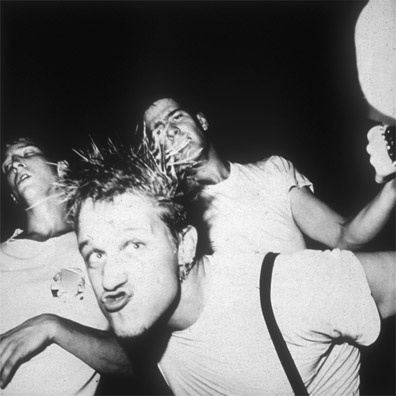
\includegraphics[width=0.4\textwidth,height=\textheight]{img/hardcore-02.jpg}

\begin{centercap}

\href{https://www.dreadscott.net/works/hardcore/}{Dread Scott}, Hardcore series, ``Devon''

\end{centercap}

\end{centerpic}

\textbf{\emph{So far we have examined}} a few different theories about the basis of ethics. Each of these theories proved inadequate for one reason or another, in spite of the fact that each one is popular. Philosophers are kind of hard to please. The failure of these theories can, however, tell us something about what an adequate ethics might look like. The first lesson we can learn from their failure is that ethical principles cannot simply be based on authority. It does not matter whether this authority is the authority of culture, a divine creator of laws, or nature -- appealing to such sources of ethical principles fails to really provide a \emph{reason} to accept those principles as legitimate. Authority may get us to act, for fear of punishment or ostracism if we fail to do what the authorities want. But authority alone will never be enough to convince us that what the authorities want us to do is right. In order to be convinced we will need to see some convincing reasons.

\textbf{\emph{Providing reasons}} to back up our claims is exactly what we do when we are attempting to be be rational. This simple observation is the point of departure for the more explicitly philosophical approach to ethics that underlies our next four approaches to ethics. These are known as egoism, social contract theory, utilitarianism and Kantian ethics. All of these approaches are products of an important period of intellectual history known as the Enlightenment. The Enlightenment was a period (which began in roughly the mid-18th century, and ended as a formal intellectual movement in roughly the mid-nineteenth century) in which intellectuals throughout the world embraced the idea that reason alone was capable of providing guidance for human affairs. According to such advocates of the Enlightenment as Thomas Jefferson, Benjamin Franklin, David Hume, Adam Smith, Jeremy Bentham and Immanuel Kant, among many others, careful and rational investigation of the world and the evidence that could be found in the world, could provide a basis for our social lives as well as scientific knowledge. There are considerable differences among the ideas of the major figures of the Enlightenment. However, all of them shared a basic trust in the power of reason to solve human problems. For egoists, social contractarians, utilitarians and advocates of Kantian ethics, rationality is the bottom line and ethics, if it is to move beyond the arbitrariness and prejudice embedded in the traditional conceptions of morality we have been considering, must embrace rationality. In the next four chapters we will be examining different answers to the question, ``What would a rational ethics look like?'' To get a sense of the territory ahead here are the answers that each of the next four approaches to ethics offers:

\begin{itemize}
\tightlist
\item
  egoism: It would not exist -- rationality requires us to put ourselves first.
\item
  social contract theory: a rational ethics would be based on an agreement about what the basic rules of the social game should be.
\item
  utilitarianism: It would be an effective method for attaining the common good.
\item
  Kantian ethics: It would be a system of universal laws that all rational agents must follow.
\end{itemize}

\hypertarget{psychological-egoism-whats-in-it-for-me}{%
\section{Psychological Egoism: What's in it for me?}\label{psychological-egoism-whats-in-it-for-me}}

\begin{epigraph}

Where the world comes in my way---and it comes in my way everywhere---I consume it to quiet the hunger of my egoism. For me you are nothing but---my food, even as I too am fed upon and turned to use by you.\\
~\\
---Max Stirner

\end{epigraph}

\textbf{\emph{Calling egoism a theory of ethics}} may seem to stretch the meaning of the word ``ethics'' to the breaking point, since egoism denies that we can or should really care about ethical rules. But since advocates of egoism make explicit claims about the relationship between ethics and rationality, any discussion of philosophical ethics cannot avoid dealing with egoism. Egoists claim, in fact, that rationality undermines the possibility of ethics as it was traditionally understood. To the extent that we follow reason, as opposed to customary authority, we will cease to be concerned with ethics. It is not that we will suddenly be cold to the needs and desires of others where we previously kept these interests close to our hearts. It is that we will recognize certain things about the way the world and human beings work that will compel us to give up certain ways of looking at the world. But I am getting ahead of myself here.

\textbf{\emph{Egoism is not a single theory,}} but two separate theories that make different, even though related, claims about human action and decision-making. These separate theories are known as ``Psychological Egoism'' and for want of a better term, ``Ethical Egoism.'' Psychological Egoism is the view that we cannot be unselfish even if we may want to be. Ethical Egoism, on the other hand, is the view that we should not be unselfish even though we can be.

\textbf{\emph{Psychological egoism}} makes a very straightforward claim: we cannot be unselfish. That is, certain facts about human psychology (hence the name Psychological Egoism), prevent unselfish, altruistic behavior from being a live option. This may sound outrageous, but defenders of PE think that there is a compelling case that can be made for this view. Note that PE is not claiming that we should not be unselfish. That is what Ethical Egoism claims and is a very different can of worms. PE presents itself as a hard-nosed and realistic view that simply reports on the way things are -- ``let's just face it, we all have an agenda, and anyone who denies this is a fool.'' According to Psychological Egoism, a careful and rational assessment of the evidence concerning human behavior, shows that ethical rules do not make very much sense, since we cannot really ever put others first. That is, ``altruism,'' (acting selflessly, putting others needs and interests before one's own) is not really possible. We will examine the arguments for this view in a moment.

\hypertarget{implications-of-psychological-egoism}{%
\subsection*{Implications of psychological egoism}\label{implications-of-psychological-egoism}}


\textbf{\emph{Clearly if PE were true,}} this would have an enormous impact on our lives. If we simply cannot ever really be unselfish, at best we are confused when we talk about ethics and and worst we are deceiving ourselves about human nature. Whatever the case may be, PE compels us to give up talking about others' needs and interests, and gives us a clear license to put ourselves first. This may sound appealing -- it relieves us from the burdens that go with ethical demands to help others, and frees us to pursue our own self-interest without the guilt feelings that society has traditionally encouraged us to feel when we put ourselves first. Furthermore, the view that we never are really unselfish strikes some people as a realistic antidote to the idealistic tone of ethics. If PE is true, describing human actions in terms of what we should and shouldn't do, in terms of duties and obligations, etc. is simply unrealistic and we should give it up. The ethical perspective would be revealed to be obsolete from the new, more realistic standpoint of Psychological Egoism. On the other hand, if PE is true, we would not really ever have any grounds for complaint about the way others treat us. If nobody really can be unselfish, what right would we ever have to ask others to take our interests seriously and not try to take advantage of us?

\hypertarget{arguments-for-psychological-egoism}{%
\subsection*{Arguments for psychological egoism}\label{arguments-for-psychological-egoism}}


These implications of PE are the kinds of things that we would have to buy, if it were true. So far we haven't been given any reason to suppose that it is in fact true. So let us take a look at the arguments that might be offered in its defense, to see if they can convince us that PE is really true. There are two main arguments in defense of PE. The first is a purely theoretical argument. It is based on an analysis of rational decision-making and claims that because of certain facts about the way we make decisions, these decisions are always selfish.

\begin{center}

\begin{argument}

When I make a decision, I am attempting to fulfill my goals since I cannot act on anyone else's goals.\\
But acting for the sake of fulfilling my goals is acting selfishly.\\
~\\
Since the same point applies equally to everyone, we are all always selfish.

\end{argument}

\end{center}

\textbf{\emph{What this argument is claiming}} is that if we think about what is involved in rational action in general, we will soon realize that it has to be selfish by definition. Since my reasons for action are my own, they must be clearly be oriented toward my own good. After all this is what it means to act rationally -- rational action is action that effectively realizes one's goals. But since these goals have to be my goals, otherwise they would fail to motivate my decisions, it clearly seems to follow that I have no choice but to act for my own sake. Acting for someone else's goals is just impossible by definition. But acting for one's own goals exclusively is just what it means to be selfish. Hence PE must be true. Wow, that was a dense bit of reasoning. If you didn't quite get it, I suggest you read it again. Maybe even read it a few times.

\textbf{\emph{A second argument}} for Psychological Egoism is an empirical argument. It does not rest on the claim that we are selfish by definition, even though that is what PE ultimately claims. Instead it appeals to evidence about real human behavior in the real world.

\begin{center}

\begin{argument}

If psychological egoism were false we should be able to find a real example of altruism.\\
But there are no real examples of altruism.\\
~\\
So psychological egoism is true.

\end{argument}

\end{center}

\textbf{\emph{Well this argument may}} just seem silly. Aren't there in fact are plenty of examples of real altruistic behavior out there? Sure some people are selfish, but there are many people who help other people at no apparent gain to themselves. Here are a few ordinary examples:

\begin{itemize}
\tightlist
\item
  A person gives all of their extra money, after paying their bills and buying groceries, to charity and does so anonymously.
\item
  Another person stops to help the victim of an accident on the highway even though doing so makes them late for an important meeting.
\item
  Someone else spends their weekends volunteering at the hospital.
\end{itemize}

\hypertarget{the-strategy-of-reinterpreting-motives}{%
\subsection*{The strategy of reinterpreting motives}\label{the-strategy-of-reinterpreting-motives}}


\textbf{\emph{As you may already suspect,}} a defender of Psychological Egoism has an answer to this objection. The second argument for PE does not instantly fall apart under the weight of these apparent counterexamples. This is because, according to PE, they are only apparent examples of altruism -- on closer examination these apparently altruistic acts can be shown to really be based on underlying selfish motives. Take the case of a person who gives to charity anonymously. Isn't there likely to be a selfish motive in this? Perhaps this person feels guilty for having as much money as she has and decides that the best way to make herself feel better is to give a large anonymous donation to a charity. Or maybe it is a way of avoiding paying taxes on the rest of her money -- if you do it right, donating to charity can save you money on your taxes by lowering your tax bracket. The same kind of argument can apply in the other cases as well. Can't we reinterpret the motives of people who help strangers in a way that makes them seem less altruistic and more selfish? Once again, the motives for helping people might be to relieve one's own guilt feelings, or to enjoy the feeling of being a hero, or the fame that goes with getting your picture in the paper as the heroic rescuer of that poor, helpless victim of the accident. Volunteering? Well, that looks great on your resume, plus it is a great way to meet people without having to buy them drinks, etc. This line of reasoning is intended to provide additional support in defense of PE against the objection that people ``obviously'' do not always act on the basis of selfish motives.

\textbf{\emph{Something may strike you}} as suspicious about this line of thinking and especially about the egoist's response to the apparent counterexamples we have just mentioned. If so, your intuitions are on the right track. It is difficult, however, to pinpoint exactly what is wrong here. In order to clarify things a bit, we need to digress for a moment and talk about the nature of empirical theories and what sorts of evidence they appeal to. This short excursion into the territory of the philosophy of science will reveal the big problem with the second argument for PE.

\textbf{\emph{If we are to have a good reason}} to accept a theory, we need some evidence to support that theory. But, how much evidence do we need? Well, it seems that the more evidence we have, the more well-confirmed our theory is and the more reason we have to believe that it is true. Suppose someone asks me to believe his theory that NASA faked the Apollo 11 moon landing. Before I buy this theory, I'll want to see the evidence. If the only evidence he offers is that he doesn't believe that such an accomplishment was possible given the primitive state of technology in 1969, I still do not have much reason to be convinced. But if more and more evidence appears to support this claim then my initial skepticism might have to give way to a belief that maybe he is right. What evidence might help convince me?

\begin{itemize}
\tightlist
\item
  A top NASA official publicly admits that the space program faked the moon landings.
\item
  Investigators find and photographically document an abandoned movie studio in the Arizona desert that is filled with exact copies of the lunar landing modules and other equipment that appeared in the original TV footage of the ``moon landing.''
\item
  Reels of film with outtakes from the TV broadcast footage are found in a warehouse in Arkansas, and this footage shows microphones and other stage equipment on the surface of the ``moon.''
\item
  The Chinese land on the moon and fail to find any evidence of a prior American landing in a thorough search of the American landing area.
\end{itemize}

\textbf{\emph{Of course no such}} real evidence like exists. The point is a more general point about how theories need to appeal to sufficient evidence if we are they are to be convincing theories. It seems that the more evidence a theory has the more believable it becomes. But there is a catch -- we shouldn't have too much evidence for a theory. Consider the following case of a theory with unlimited evidence, the theory that there is a massive conspiracy against me personally. I might mention the following evidence in support of this theory:

\begin{itemize}
\tightlist
\item
  The person who almost ran me over when I was walking across the street this morning is clearly in on the conspiracy.
\item
  Yesterday I asked someone if they were in on the conspiracy against me, and they nervously replied ``Of course not.'' Obviously a lie!
\item
  Even my best friend laughed when I asked him, and then admitted to being in on the conspiracy.
\end{itemize}

\textbf{\emph{I could go on}} mentioning more and more ``evidence'' for this theory, otherwise known as ``paranoia.'' And in fact, if I were in the grip of genuine paranoia, I would have an unlimited amount of evidence at my disposal. Whatever counterexamples anyone could come up with to try to calm my fears could easily be explained away as still more evidence in favor of the conspiracy against me. Clearly there is a problem here. The problem with paranoia, considered as an empirical theory -- a claim about what is really going on in the world -- is not that there is no evidence for it. Instead, the problem is that there is no possible evidence that might count against it. In philosophical jargon it is ``non-falsifiable.''

\textbf{\emph{All empirical theories}} not only need evidence to support them, they also need to be falsifiable, that is, there has to be at least the possibility that they are wrong. Note that ``falsifiable'' does not mean the same thing as ``false,'' or ``falsified.'' Such theories are obviously no good -- they have failed the tests that we have given them and should be rejected. Falsifiable theories are theories that might not be true, even if the only such theories that are worth our time are ones that have not yet been shown to be false. But legitimate theories have to be at least capable of being tested with tests that they might possibly fail. After all, if the only tests you give a theory are tests that it cannot possibly fail, have you really learned anything new about anything by testing your theory? In fact it is better to say that non-falsifiable theories are not even really theories that make claims about how the world really is -- instead they are assumptions that we project onto the world with no evidence whatsoever.

\textbf{\emph{To return to Psychological Egoism,}} it now appears that this too is a non-falsifiable theory, just like paranoia. The ``tests'' that the theory was given in our discussion above were the apparent counterexamples -- cases where it appears that people are in fact not operating based only on selfish motives. PE of course had a ready answer to all of these challenges -- all we have to do is come up with some possible hidden motive that explains away the appearance of altruism and the theory is back in business. But this is a game that the defender of PE cannot possibly lose. We can always reinterpret others' motives in way that undermines the appearance of altruism. As a result, however, PE loses any claim it may have had to be a genuine theory about what human behavior is really like and is revealed to be nothing but a cynical projection of selfish motives onto all human action. The strategy of reinterpreting motives, which seemed like a promising way to defend PE, in fact renders it non-falsifiable and hence empty of real empirical content. It reveals nothing about the world, but everything about the assumptions of the person defending this ``theory.''

\textbf{\emph{But what about}} the first argument? This argument claimed that we could see that human behavior has to be selfish to the extent that it is rational simply because we all are only capable of making decisions that fulfill our own goals. Rational decision-making is decision-making that realizes one's own goals and so is bound to be selfish. A little reflection on this argument reveals a subtle problem. Does the fact that a goal is my own goal have to mean that my interests alone are at stake in the attempt to satisfy that goal? Only if we assume that I cannot have goals that involve helping other people. But why should we assume this? PE claims that my goals are always my goals, and so they must be selfish. But doesn't this mix up two different meanings of the expression ``my goals.'' Clearly it is true that my goals are my own -- if they are going to get my body moving, they have to be in my own head. That is a trivial truth of human psychology -- it is so obvious that there usually isn't much point mentioning it. The thoughts in your head cannot cause me to do anything, at least in any direct way. But ``my goals'' might also mean, ``my goals, as opposed to your goals'' in a situation where both cannot be satisfied simultaneously. If my goal is to rob you of all of your money and your goal is to prevent me from doing that this is the meaning of the expression ``my goals'' that is appropriate. But these two meanings are different, so if our argument uses both of these meanings as if they were equivalent, it is guilty of the fallacy of equivocation. Thus the first argument is revealed to be invalid, since it equivocates on the meaning of the expression ``my goals.''

\textbf{\emph{Thus we can see}} that both arguments for PE ultimately fail. As a result, however cynical we may sometimes feel about the possibility of genuine altruism, we must leave open the possibility that we are at least capable of being altruistic. Whew! It takes philosophers an enormously long time to establish the simplest of points. Well, at least we can now respond definitively to the cynics who assert that by definition everything we do is selfish.

\hypertarget{ethical-egoism}{%
\section{Ethical Egoism}\label{ethical-egoism}}

\textbf{\emph{Given that human action}} might be unselfish in some cases, we may still wonder whether we ever really have any good reasons to act unselfishly. Is selfishness ethically defensible? If we consider may peoples' actions, it appears that human beings can be pretty selfish. Consider for example, the former CEO of Tyco, Inc., L. Dennis Kozlowski. He and another executive engaged in massive fraud, stealing hundreds of millions of dollars from investors and employees of his firm -- all so he could live a life of excessive luxury, which included paying \$6000 for a shower curtain with gold threads woven into it and spending well over \$2 million on a birthday party for his wife.

\textbf{\emph{Such behavior seems}} patently wrong. But on what grounds can we say this? Defenders of Ethical Egoism claim that in fact we have no real grounds for condemning such behavior, because the only duties we really have are to ourselves. If we had the opportunity and thought we could get away with it, we'd really act no differently than Kozlowski, and we needn't feel guilty about it either.

\textbf{\emph{Ethical Egoists claim}} that we should always put ourselves first and that we should refrain from helping other people. This view differs from Psychological Egoism since PE makes a descriptive claim -- it describes what human actions are really like -- while EE is makes prescriptive claims -- it tells us what we should be doing whatever it is that we happen to be doing in reality. Because of this, EE is not going to appeal to facts about human psychology, but is going to try to show why it is that selfishness is better than altruism in general. Of course, arguing that selfishness is better for me is easy, so defenders of EE will need to appeal to deeper reasons in order to show why it is that selfishness is better for everybody.

\hypertarget{implications-of-ethical-egoism}{%
\subsection*{Implications of ethical egoism}\label{implications-of-ethical-egoism}}


\textbf{\emph{Before we get to the reasons}} that might be offered in defense of selfishness, we should be clear on where this view leads us. Even more so than Psychological Egoism, Ethical Egoism would give us a license to act selfishly. So, for example, even though people in rich countries could very easily save the lives and end the misery of millions of people in poor countries just by sending a little extra cash to charitable organizations and not spending it on needless luxuries, relatively few people actually do this. According to EE, there is absolutely nothing wrong with this. If you want to send your money to people less well-off, by all means that is your right. But it is certainly not your duty to do so. This may sound pretty cold, and perhaps it is. But us philosophers really only care about whether it is a rationally defensible position. If it is, then we will just have to learn to live with the implications.

\hypertarget{in-defense-of-ethical-egoism}{%
\section{In defense of ethical egoism}\label{in-defense-of-ethical-egoism}}

\textbf{\emph{OK, so what reasons}} might be given to support the idea that we have no real duties towards others, that we can and even should always put ourselves first? There are three main arguments to consider here, which I'll call ``Rand's argument,'' ``the capitalists' argument,'' and ``the revisionist argument.''

\textbf{\emph{The first argument}} we'll examine was developed by the Russian emigre philosopher and novelist named Ayn Rand (1905-1982). Rand was a staunch opponent of communism who dramatised her ideas in the best-selling novels The Fountainhead and Atlas Shrugged, as well as in essays with titles such as ``The Virtues of Selfishness.'' Her argument for EE goes like so,

\begin{center}

\begin{argument}

What makes human life valuable is its individuality.\\
Fulfilling yourself as an individual requires putting your own needs and interests first.\\
Altruistic behavior involves sacrificing your own interests for those of other people.\\
~\\
So acting ethically should be avoided since it undermines what makes human life valuable.

\end{argument}

\end{center}

\textbf{\emph{That is, we should be wary}} of the ethical demand for self-sacrifice since this undermines what is truly valuable about human lives. This is exactly what happened in communist countries -- individuals were asked to sacrifice their own selfish desires and interests for the good of the whole and in the end they got nothing for their sacrifices, while the leadership who demanded these sacrifices accumulated power and privileges it denied to everyone else.

\textbf{\emph{The second argument}} for EE is an argument that you have probably heard before. It is commonly used in defense of cutting government social spending, privatizing governmental institutions and getting rid of welfare programs. I call it ``the capitalists' argument'' and it goes like so:

\begin{center}

\begin{argument}

If we help others we are undermining competition and all of the good that competition produces.\\
Market forces, what Adam Smith called ``the invisible hand'' of free markets, act in such a way as to determine the best possible distribution of social goods.\\
~\\
Interfering with such forces may seem to be benevolent, but in the end it will only lead to some people taking advantage of benevolence and everybody losing out from the loss of the benefits of competition.

\end{argument}

\end{center}

\textbf{\emph{The last argument in favor}} of Ethical Egoism alleges that when properly understood, all ethical rules really express appeals to our self-interest. Ethical rules make sense because they work for each of us. I call this a ``revisionist'' argument because it reinterprets or revises the content of ethical rules so that they look just like rules any self-interested agent would accept. Ethics is not a challenge to self-interest, but an expression of self-interest. The argument might run like so:

\begin{center}

\begin{argument}

Ethical rules can be rephrased in terms that appeal to self-interest.\\
For example, ``Lying is wrong,'' really means ``It is in your best interest not to lie;'' ``Murder is wrong'' really means ``Life is better for you if you refrain from murdering people.''\\
~\\
So defending ethical rules is really defending selfishness.

\end{argument}

\end{center}

\textbf{\emph{This argument equates ethics with}} the pursuit of self-interest, so that whether you happen to defend acting ethically or not, you are still always defending acting in a self-interested way.

\textbf{\emph{What are we to}} make of these arguments? Do they really present a convincing case that we should turn our backs on the demands of others, that we should guiltlessly pursue our own interests? Let us consider them more carefully one at a time.

\textbf{\emph{Rand's argument}} is essentially that ethics in the traditional sense of a set of commands that require us to put others first is incompatible with genuine concern for human individuality and with individuals' truly achieving their personal goals. That is, to the extent that we contribute to the welfare of others, we are required to give up our own welfare. But is this really true? It would be true if human social life were a ``zero sum game'' where my gain is only possible if others lose an equal amount. Poker is a good example of a zero sum game in which it makes no sense to act benevolently towards others. If I am playing poker I am playing to win money from others -- their loss is my win and vice versa. But is life in society really like a poker game in which I have to take from others in order to win? Aren't there ever any benefits to all (and each) from cooperating, from setting aside immediate gains for the sake of a greater collective good? Of course there are. For example, a number of investors might pool their resources to open up a business that benefits all of them much more than if each had simply stolen the others' contributions. This is possible since valuable goods can be created when we work together. Unlike in poker, where there is a fixed pool of money that is divided among the players in the end, in society we can use our given resources to make more things of value than we started with. Thus Rand's argument proves in the end to be unsound, since the second and third premises are just false -- fulfilling yourself as an individual does not require putting your own needs and interests first, and altruistic behavior might not have to require a complete sacrifice of your own interests.

\hypertarget{capitalism-and-the-common-good}{%
\section{Capitalism and the common good}\label{capitalism-and-the-common-good}}

\textbf{\emph{So, what then}} about the capitalist's argument that we should practice ``tough love,'' and not help others in order to encourage them to help themselves? In certain situations this seems like the best way to get the best outcome for all of us -- if I run a business in a competitive industry, I will be forced by market forces to produce the best products for prices that people will want to pay, and that make me enough of a profit to want to stay in business. I want what is best for me -- profits -- and my customers want what is best for them -- products that are of acceptable quality and cost for their needs. So selfish individual behavior can lead to an overall outcome that is best for all of us. So far so good. There are two problems, however, with this argument. The first is that competition is not always the best way of producing the best outcome for all involved. In some industries competition helps both the producer and the consumer -- competition forces the producer to keep prices lower and quality higher. But is this the case in all markets? What about, for example, health care? If we opened up health care to free competition this would mean that hospitals and other health care providers would be offering a service to consumers for the sake of making profits. If the consumer was dissatisfied with the services offered she could just go elsewhere next time and this would encourage health care providers to lower prices and increase the quality of their services. This all sounds good, until we realize that there is something very different between consumer goods and health care services. When I am sick, I often do not have the time or the ability to shop around for the best health care -- I need help now. And if I am not satisfied with the poor services offered to me at one hospital as treatment for my illness, I may not get the chance to go elsewhere next time, since there may be no next time. So, and this is a technical point that probably needs much more development to be thoroughly convincing, not all social institutions would be benefit from being opened up to competition, even if in certain cases competition is beneficial.

\textbf{\emph{There is, however}} a deeper problem with the capitalist's argument for egoism. Granted that at times competition for selfish gain leads to a better outcome for all of us, we may wonder why an egoism -- someone who claims that selfishness is acceptable -- even cares about the good of everyone. If we are defending egoism, doesn't it seem strange to base our argument on a concern for others? Can we even really be defending selfishness in this way? If we claim that selfish behavior can produce good outcomes for all of us, then we are putting our selfish impulses to work for society and not subordinating social concerns to selfish concerns. So calling this argument an argument for egoism is really incoherent, it makes no sense to be claiming that we should always be selfish because that is the way to insure that everyone benefits.

\textbf{\emph{Finally, we have}} the last argument for Ethical Egoism to deal with. This argument claimed to establish that we should always be selfish because even ethical rules only really encourage us to do what is in our self-interest anyway. I called this the ``revisionist argument'' since it tries to revise ethical rules in a way that turns them into rules that even purely self-interested people would be willing to accept. The problem here is that when we revise ethics in this way, we lose something important about ethical rules. It might be nice if ethical rules were things that even the most self-involved people among us could easily live with, but unfortunately that is not the case. Ethics makes demands on us that we can't always just simply accept. For example, even though at times refraining from lying is really in my own best interest, since it helps to maintain trust between myself and others upon whom I rely to tell me the truth, this is not always the case. If there is an ethical rule about usually not lying, it is because at times it probably seems to me that it is in my selfish interest to lie to others, even if there are larger reasons not to lie. Ethical rules frequently ask us to set our self-interest aside for the sake of larger goals or purposes. Of course, we have not yet seen why we should ever do this (utilitarianism and Kantian ethics, as we will see, offer two different arguments why we should). But to claim that ethics does not ever really do this is to throw out the proverbial baby with the bath water. If ethics is really reducible to self-interest, merely throwing out those parts of ethics that conflict with self-interest is no way to show this. And all we have to do to seem that it is probably not reducible in this way to consider any situation in which ethics makes demands on us not to do something that it is in our self-interest to do.

\hypertarget{further-exploration-4}{%
\section*{Further exploration}\label{further-exploration-4}}


\hypertarget{social-contract-theory}{%
\chapter{Social Contract Theory}\label{social-contract-theory}}

\begin{centerpic}


\includegraphics[width=0.5\textwidth,height=\textheight]{img/constitution.jpg}

\begin{centercap}

\href{https://pixabay.com/users/lynn0101-8308820/}{lyn0101} at Pixabay.com

\end{centercap}

\end{centerpic}

\begin{epigraph}

For it can never be that war shall preserve life, and peace destroy it.\\
~\\
---Thomas Hobbes, Leviathan

\end{epigraph}

\hypertarget{hobbes-and-the-invention-of-society}{%
\section{Hobbes and the invention of society}\label{hobbes-and-the-invention-of-society}}

\hypertarget{the-prisoners-dilemma}{%
\section{The Prisoners Dilemma}\label{the-prisoners-dilemma}}

\hypertarget{why-should-we-follow-the-rules}{%
\section{Why should we follow the rules?}\label{why-should-we-follow-the-rules}}

\hypertarget{utilitarianism}{%
\chapter{Utilitarianism}\label{utilitarianism}}

\begin{centerpic}


\includegraphics[width=0.5\textwidth,height=\textheight]{img/crowd.jpg}

\begin{centercap}

\href{https://pixabay.com/users/free-photos-242387/}{Free-Photos} at Pixabay.com

\end{centercap}

\end{centerpic}

\begin{epigraph}

Actions are right in proportion as they tend to promote happiness, wrong as they tend to produce the reverse of happiness.\\
~\\
---John Stuart Mill, Utilitarianism

\end{epigraph}

\hypertarget{the-highest-good}{%
\section{The highest good}\label{the-highest-good}}

\hypertarget{why-should-i-care}{%
\section{Why should I care?}\label{why-should-i-care}}

\hypertarget{problems-problems}{%
\section{Problems, problems}\label{problems-problems}}

\hypertarget{kant-and-the-ethics-of-duty}{%
\chapter{Kant and the ethics of duty}\label{kant-and-the-ethics-of-duty}}

\begin{centerpic}


\includegraphics[width=0.55\textwidth,height=\textheight]{img/king-audacity.jpg}

\begin{centercap}

\href{https://www.flickr.com/photos/22711505@N05/}{Ron Cogswell}

\end{centercap}

\end{centerpic}

\begin{epigraph}

Two things fill the mind with ever-increasing wonder and awe, the more often and the more intensely the mind of thought is drawn to them: the starry heavens above me and the moral law within me.\\
~\\
---Immanuel Kant, Critique of Practical Reason

\end{epigraph}

\hypertarget{what-do-we-owe-one-another}{%
\section{What do we owe one another?}\label{what-do-we-owe-one-another}}

\hypertarget{the-categorical-imperative}{%
\section{The Categorical Imperative}\label{the-categorical-imperative}}

\hypertarget{rights-and-duties}{%
\section{Rights and duties}\label{rights-and-duties}}

\hypertarget{references}{%
\chapter*{References}\label{references}}


\hypertarget{refs}{}
\leavevmode\hypertarget{ref-BayPigsGroupthink}{}%
``Bay of Pigs - Groupthink.'' Accessed December 2, 2019. \url{https://www.globalsecurity.org/intell/ops/bay-of-pigs-groupthink.htm}.

\leavevmode\hypertarget{ref-benedictPatternsCulture1935}{}%
Benedict, Ruth. \emph{Patterns of Culture}. Boston and New York: Houghton Mifflin, 1935.

\leavevmode\hypertarget{ref-davisWouldYouPull2015}{}%
Davis, Lauren Cassani. ``Would You Pull the Trolley Switch? Does It Matter?'' The Atlantic, 2015. \url{https://www.theatlantic.com/technology/archive/2015/10/trolley-problem-history-psychology-morality-driverless-cars/409732/}.

\leavevmode\hypertarget{ref-gelmanEssentialismEverydayThought}{}%
Gelman, Susan. ``Essentialism in Everyday Thought.'' American Psychological Association. Accessed December 13, 2019. \url{https://www.apa.org/science/about/psa/2005/05/gelman}.

\leavevmode\hypertarget{ref-gilovichHowWeKnow1991}{}%
Gilovich, Thomas. \emph{How We Know What Isn't So}. New York: The Free Press, 1991.

\leavevmode\hypertarget{ref-kahnemanThinkingFastSlow2011}{}%
Kahneman, Daniel. \emph{Thinking Fast and Slow}. New York: Farrar, Straus and Giroux, 2011.

\leavevmode\hypertarget{ref-lentPatterningInstinct2017}{}%
Lent, Jeremy. \emph{The Patterning Instinct}. Amherst, NY: Prometheus Books, 2017.

\leavevmode\hypertarget{ref-prestonMooreGeorgeEdward}{}%
Preston, Aaron. ``Moore, George Edward.'' Internet Encyclopedia of Philosophy. Accessed December 13, 2019. \url{https://www.iep.utm.edu/moore/}.

\end{document}
